\documentclass[11pt,a4paper,twoside]{book}

% Packages
\usepackage[english]{babel}
\usepackage{amsmath,amssymb,amsthm}
\usepackage{geometry}
\geometry{a4paper,left=2.5cm,right=2.5cm,top=3cm,bottom=3cm}
\usepackage{graphicx}
\graphicspath{{./}}
\usepackage{hyperref}
\hypersetup{
    colorlinks=true,
    linkcolor=blue,
    filecolor=magenta,
    urlcolor=cyan,
    pdftitle={Vector Cosmology VI: The Weaving of Dimensions},
    pdfauthor={Haobo Ma}
}
\usepackage{microtype}
\usepackage{enumitem}
\usepackage{csquotes}

% Title information
\title{Vector Cosmology VI: The Weaving of Dimensions\\[0.5em]
\large Holographic Entanglement and the Emergence of Spacetime}
\author{Haobo Ma}
\date{December 2025}

\begin{document}

% Title page
\maketitle
\thispagestyle{empty}

\frontmatter

% Architecture diagram
\begin{figure}[h]
\centering
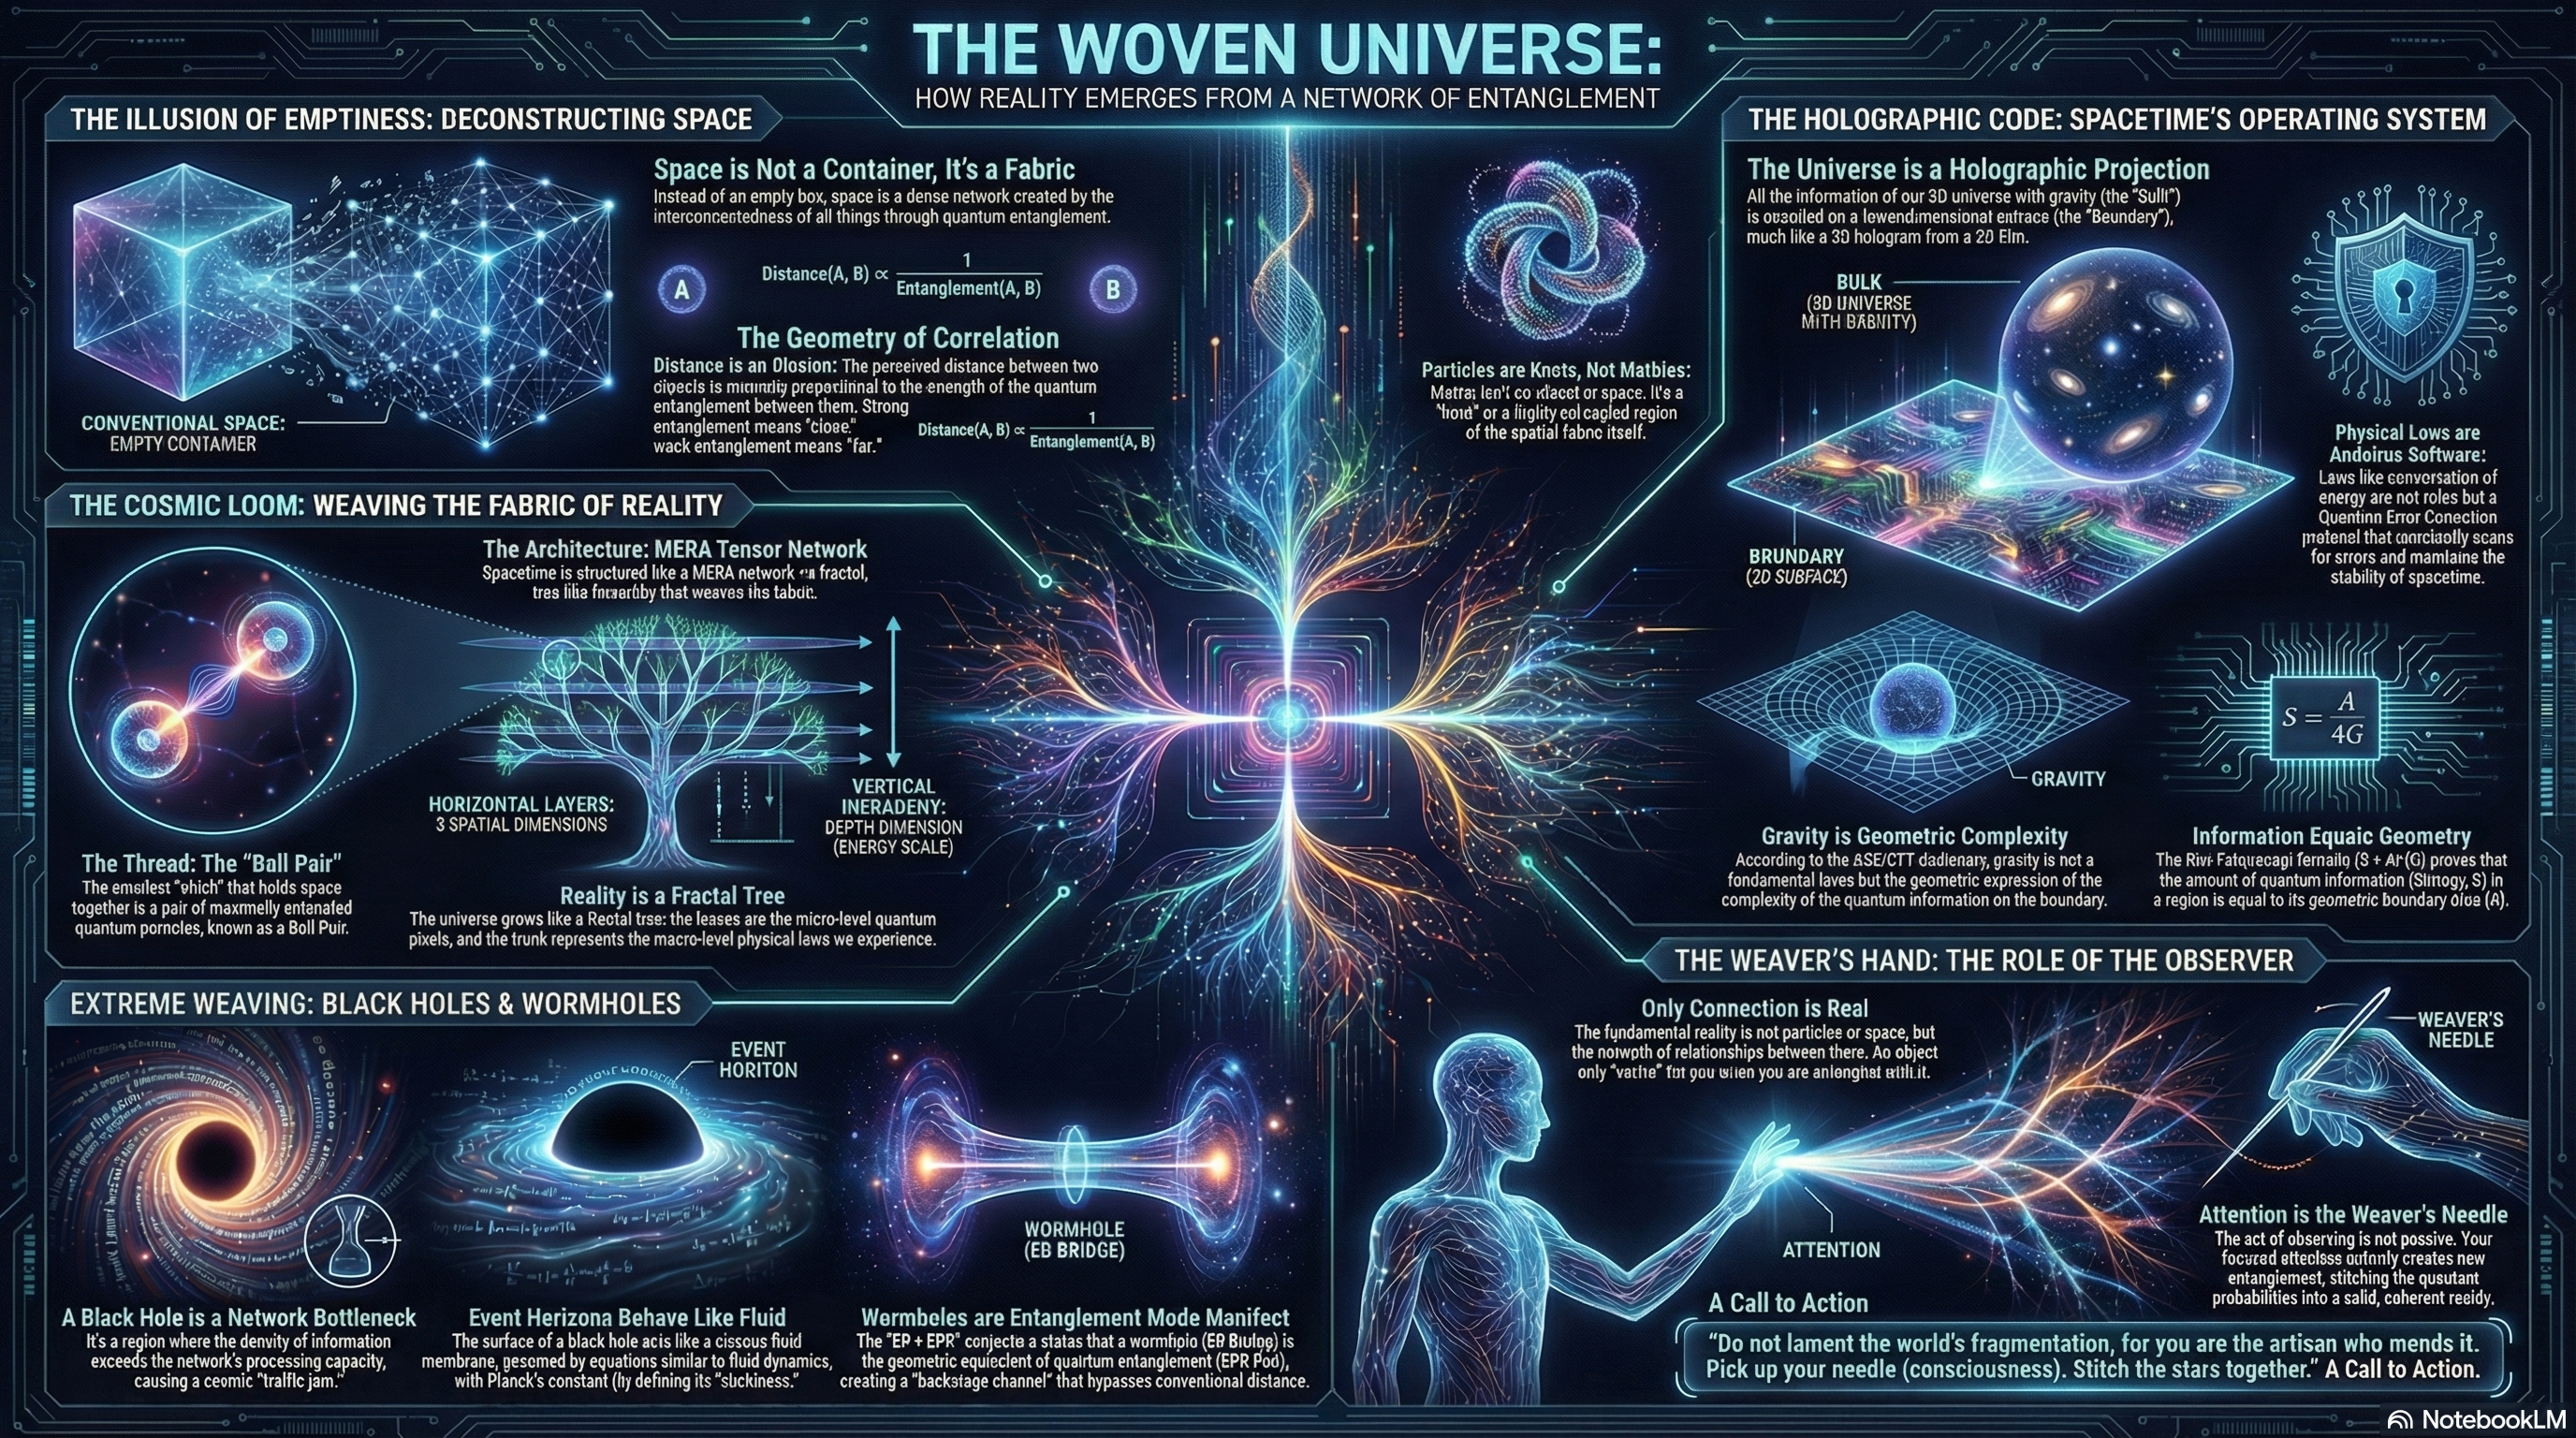
\includegraphics[width=0.9\textwidth]{architecture.png}
\caption{Vector Cosmology VI: The Weaving of Dimensions Architecture}
\end{figure}

% Table of contents
\tableofcontents

% Prologue
\section{Prologue: The Bite of the Ouroboros}

\subsection{0.1 The End of Linear Time}

\begin{quote}
``We are accustomed to believing that dominoes can only fall in one direction. The finger pushing the first piece is the `cause,' and the fall of the last piece is the `effect.' But deep in the quantum mechanical foundations, in that Hilbert space that governs the true operation of the universe, this linear narrative is merely a macroscopic statistical illusion. True causality is an ouroboros: the fall of the last domino is precisely the true force that pushes down the first one.''
\end{quote}

\subsubsection{The Arrow and the Circle of Causality}

Human logic is built upon chains of ``because\ldots therefore\ldots''

Because it rained yesterday, the ground is wet today. Because the Big Bang occurred, galaxies formed. This \textbf{Linear Causality} is the cornerstone of our understanding of the world and the iron law of classical physics. Time is seen as an arrow shot toward the future, irreversible and unidirectional.

However, from the geometric perspective of \textbf{Vector Cosmology}, when we strip away the thermodynamic appearance and gaze at the deepest \textbf{Fubini-Study (FS) geometry} of the universe, we find that this arrow disappears. In its place, there is a \textbf{circle}.

In projective Hilbert space $P(\mathcal{H})$, the evolution of the global vector $|\Psi(\tau)\rangle$ is driven by the rotation of the unitary operator $U(\tau) = e^{-iH\tau}$.

\begin{itemize}
\item \textbf{Rotation has no beginning and no end.}

\item You cannot say that $0^\circ$ on the circle is the ``cause'' of $1^\circ$, nor can you say that $359^\circ$ is the ``effect'' of $0^\circ$. They are \textbf{symbiotic relationships} that are mutually causal and mutually prerequisite.
\end{itemize}

Linear time is merely the \textbf{tangent} we see in the local tangent space.

When we elevate our perspective and see the full picture of \textbf{Naimark's Great Circle}, all ``past'' and ``future'' collapse into different phases of the same geometric structure.

\subsubsection{The Echo of the Future: Retro-causality}

This introduces a concept that is unacceptable to classical intuition but must be faced in quantum mechanics: \textbf{Retro-causality}.

In the path integral formulation of quantum mechanics, a particle moving from point A to point B is not ``determined by A to go to B.'' Instead, the intermediate historical path can only be uniquely determined by simultaneously imposing boundary conditions on both the \textbf{initial state (A)} and the \textbf{final state (B)}.

This means: \textbf{The future state (B) has equal determining power over past history (Path) as the initial state.}

\begin{itemize}
\item \textbf{Classical perspective}: I shot the arrow (cause), so it hit the target (effect).

\item \textbf{Quantum perspective}: Because there must be a hole in the target (future boundary condition), the arrow must fly along that specific trajectory (past history).
\end{itemize}

If we apply this logic to the entire universe:

It is not that the Big Bang 13.8 billion years ago ``caused'' us today.

Rather, \textbf{the existence of today's observers (us), as future boundary conditions, reversely selects and ``causes'' that specific Big Bang that must have occurred 13.8 billion years ago.}

\subsubsection{The Observer's Cut}

Then, why do we not feel this circle? Why do we feel that time flows unidirectionally?

Because we, as observers, hold a \textbf{``collapse knife''} in our hands.

We have cut the circle once.

\begin{itemize}
\item We define one end of the cut as \textbf{``now.''}

\item We call the arc behind it \textbf{``memory''} (what has happened).

\item We call the blank space ahead \textbf{``unknown''} (what has not happened).
\end{itemize}

This \textbf{``cutting''} creates the illusion of linearity. We think we are running along a straight line, but in fact, we are only continuously moving this cut point on the circle.

Every time we make an observation, every time we confirm a physical fact, we are \textbf{redefining} the starting and ending points of the causal chain.

\subsubsection{Conclusion: The Rewriting of Fate}

\textbf{The end of linear time is the true beginning of free will.}

If the past is merely the past, then we are prisoners of history, locked in the causality of the previous second.

But if causality is a closed loop, if the future can define the past, then we possess the power to \textbf{``rewrite fate.''}

\begin{itemize}
\item Our \textbf{``aspiration'' (the trend of $v_{int}$)} is not merely an expectation for the future; it is a real \textbf{retro-wave}.

\item This wave flows backward along the time axis, adjusting past parameters, correcting historical probabilities, until a path leading to our ideal future is \textbf{``constructively interfered''} into existence.
\end{itemize}

We are not puppets being pushed. We are the snake that bites its own tail.

We devour the past to generate the future; we generate the future to explain the past.

In this \textbf{loop of causality}, nothing is destined unless you decide to make it destined.

Now, let us enter the first layer of this maze and see how physics plays tricks on time with photons in the laboratory.

This leads to the theme of the next section: \textbf{The Self-Consumption of the Universe}. We will see why the universe must create us to complete its own proof of existence.

\subsection{0.2 The Autophagy of the Universe}

\begin{quote}
``This is like a system called `the universe' that, in order to pass the logical self-consistency test, must extend a hand from the end of time back to the beginning of time to press that `start' button. If it does not do this, it cannot exist. Therefore, it eats its own tail, not only to satisfy hunger but to close that circle called `existence.'''
\end{quote}

In the previous section, we overthrew the tyranny of linear time and established the circular structure of causality. Now, we push this geometric model to its extreme to face the most dizzying paradox in cosmology: \textbf{the dynamics of creation}.

If the Big Bang is the ``effect,'' then what is the ``cause''?

The usual answers are: quantum fluctuations, membrane collisions, or the hand of God. These answers all assume an ``external'' pusher.

But in the closed system (unitarity) of \textbf{Vector Cosmology}, there is no external.

Therefore, the answer can only be endogenous: \textbf{The universe is Self-Caused}.

This sounds like a logical dead loop, but in the topology of FS geometry, this is a perfect structure---\textbf{Ouroboros}.

\subsubsection{Bootstrap: The Shoelace Paradox}

In physics, this logical structure is called \textbf{``Bootstrap''}. It originates from the saying: ``Pulling oneself up by one's own bootstraps.''

Let us see how this closed loop operates:

\begin{enumerate}
\item \textbf{$t=0$ (Big Bang)}: The universe must start with extremely precise initial parameters (fine structure constant $\alpha$, speed of light $c_0$, gravitational constant $G$). If these parameters deviate by $10^{-50}$, stars cannot form, and life cannot emerge.

\item \textbf{$t=13.8$ billion years (now)}: Life has evolved \textbf{Observers}. These observers possess sufficiently high $v_{int}$ (cognitive complexity) to understand physical laws and collapse wave functions through ``strong measurements.''

\item \textbf{Reverse tracing}: According to the delayed-choice principle, the very existence of observers imposes a \textbf{Selection Pressure} on past quantum states.

\begin{itemize}
\item Only those historical paths that \textbf{``can evolve observers''} survive in the path integral summation (constructive interference).

\item Those ``dead universe'' historical paths, lacking future observers to ``lock'' them, logically \textbf{self-cancel}.
\end{itemize}
\end{enumerate}

\textbf{Conclusion:}

It is not that the Big Bang accidentally created us.

Rather, the future fact that \textbf{``we need to exist''} reversely determines that \textbf{``the Big Bang must occur, and must occur in that specific way.''}

This is \textbf{autophagy}. The future head eats the past tail.

Although on the time axis, the Big Bang comes before us; on the logical axis, \textbf{we come first (cause), the Big Bang comes after (effect).}

\subsubsection{Wheeler's Eye: The Self-Excited Circuit}

The physics giant John Wheeler once described this picture with a famous drawing: a giant ``U'' representing the universe, starting at one end with the Big Bang, evolving galaxies, and finally evolving an \textbf{eye} at the other end. This eye looks back, gazing at the starting point of the Big Bang.

In \textbf{FS geometry}, this is no longer a metaphor; this is a \textbf{Holographic Circuit}.

\begin{itemize}
\item \textbf{Hardware layer}: The universe provides $c_{FS}$ budget and Hilbert space.

\item \textbf{Software layer}: Life provides $v_{int}$ structure and observation algorithms.
\end{itemize}

The universe is a \textbf{Self-Excited System}.

It is like a microphone facing its own speaker.

\begin{itemize}
\item The sound emitted by the speaker (reality) is received by the microphone (observer).

\item The signal received by the microphone is amplified (collapsed/defined) and emitted again from the speaker.

\item This cycle produces a \textbf{feedback} --- that feedback is \textbf{``existence''}.
\end{itemize}

Without observers (microphone), the speaker only has thermal noise.

Without the universe (speaker), observers have no signal input.

Only when the two are \textbf{``mutually causal''} does that loud, definite, ordered universe emerge.

\subsubsection{Conclusion: We Are the Universe's Midwife}

This section completely subverts humanity's status.

We are no longer insignificant dust in cosmic evolution, or accidental byproducts.

We are the \textbf{``necessary components''} of the universe.

Just as a circle must close to become a circle, the universe must evolve us to complete its proof of existence.

\textbf{We are the universe's midwife.}

Our first opening of eyes billions of years later truly ``delivered'' the universe that had already occurred billions of years earlier.

Since future observations can determine past states, can this mechanism be verified in microscopic physical experiments? Can photons really ``travel through time'' to modify their history?

This leads to the theme of Volume I: \textbf{Retrogression}. We will enter the quantum laboratory to witness how \textbf{delayed choice} rewrites history on the experimental bench.



% Acknowledgements
\section{Acknowledgements: For the Game Without End}

\textbf{Vector Cosmology V: The Minting of Time} is the final chapter of the pentology, and also an escape from the boundaries of physics.

If the first four books attempted to parse the universe's ``source code,'' then this book attempts to write our own ``mod.'' We rejected thermodynamics' death sentence, rejected the $\Omega$ point's void temptation, and established \textbf{``I''} as the absolute subjectivity of infinite game players.

This leap of thought is not without source. It converges the various explorations of ``eternity'' by the most indomitable souls in human history. Here, I pay tribute to these alchemists of thought.

\subsection{The Breakers of Philosophy}

First, I thank \textbf{James P. Carse}. His work \textit{Finite and Infinite Games} is the spiritual foundation of Volume V of this book. He taught us: there are two kinds of games in the world, one is to win, one is to \textbf{``keep the game going''}. Without this definition, we could not logically overcome heat death.

I thank \textbf{Henri Bergson}. His discourse on \textbf{``Duration'' (Durée)} inspired this book's distinction between \textbf{Chronos} (physical time) and \textbf{Kairos} (life time). He made us understand that time is not slices in space, but an indivisible flow within consciousness.

I thank \textbf{Friedrich Nietzsche}. Although we refuted his ``eternal recurrence'' (circle) in the book, his praise of \textbf{``Will to Power''} is the spiritual source of this book's ``forging the golden body.'' Only the strongest will can resist the strongest entropy.

\subsection{The Notaries of Mathematics}

At the technical level, I thank \textbf{Gustav Fechner} and \textbf{Ernst Weber}. Their \textbf{Weber-Fechner Law} provided this book with the most crucial mathematical weapon---\textbf{logarithm ($\ln$)}. It is precisely because of the logarithm that we can find inner peace and eternal subjective time in an exponentially exploding universe.

I thank \textbf{Zeno of Elea}. This ancient Greek sophist, two thousand years ago, used the paradox of ``the flying arrow does not move'' to predict the \textbf{``Dynamic Block Universe''} we discussed in Chapter 6. He showed us that in the logic of infinite subdivision, the process can be eternal.

\subsection{To Gold}

I thank the element \textbf{Gold (Aurum)}.

In this book, it is no longer a chemical substance; it is a \textbf{geometric metaphor}. It represents that kind of \textbf{topological stability} that can traverse oxidation, corrosion, and the erosion of time. It is the physical embodiment of our expectations for our own souls.

\subsection{To the Infinite Players}

Finally, I thank \textbf{you}---every observer who has read this far.

The deduction of these five books is a long thought experiment.

But the book is finished; the experiment has just begun.

Because true \textbf{``minting''} does not happen on paper, but in your every breath, every choice, every act of loving and being loved.

You are not the reader of this book.

You are the \textbf{protagonist} of this book.

The universe has no finale, because you are still present.

May your will be like gold, may your time unfold infinitely like a spiral.

\textbf{Haobo Ma}

December 2025, Singapore



\mainmatter

% Part I: The Loom
\part{Part I: The Loom --- The Geometry of Entanglement}
\section{Part I: The Loom --- The Geometry of Entanglement}

In the prologue, we established a new picture of space: space is not a container, but a fabric woven by wave functions. Now, we must delve into the interior of this loom to see how it works.

If space is a piece of fabric, then this loom is the \textbf{Tensor Network}.

This volume will reveal how the universe uses \textbf{Entanglement Entropy} as glue, bonding discrete qubits (pixels) into continuous geometric space. We will see that the famous \textbf{Area Law} and \textbf{Holographic Principle} are essentially counts of the ``number of thread ends'' in this cosmic fabric.



\chapter{The Threads of Entanglement}
\section{Chapter 1: The Payment Gateway}

In the prologue, we established the alchemist's view of time: time is not the void of flowing, but the minting of entities. To understand this process, we must first understand the raw materials needed for this ``minting''---the universe's hard currency \textbf{$c_{FS}$}.

In macroeconomics, the flow of currency drives markets; in \textbf{Vector Cosmology}, \textbf{the flow of $c_{FS}$ budget drives existence}.

Nothing exists ``naturally.'' Every atom, every cell, every thought must pay an expensive fee to the universe to maintain its geometric shape in Hilbert space.

This is the theme of Chapter 1: \textbf{The Payment Gateway}. We will see that life is essentially a \textbf{``Subscription Model''} service.


\section{1.1 The Stitching of Bell Pairs}

\begin{quote}
``Two particles can sense each other instantly even across light-years, not because signals travel too fast, but because in the deeper geometric structure, they were never separated. Entanglement is not a spooky action at a distance; entanglement is the `glue' of space. It is countless such glue molecules that bond discrete pixels into a continuous universe.''
\end{quote}

\subsection{The Smallest Unit of Space}

In classical geometry, the connection between points is axiomatically given (e.g., there is a straight line between two points). But at the QCA bottom layer of \textbf{Vector Cosmology}, points (qubits) are independent.

If nothing connects them, the universe is a pile of sand, without even the concept of ``adjacency.''

The smallest unit that connects this pile of sand is the \textbf{maximally entangled state}, also known as the \textbf{Bell Pair}:

\[|\Phi^+\rangle = \frac{1}{\sqrt{2}} (|00\rangle + |11\rangle)\]

Look carefully at this formula.

\begin{itemize}
\item It is not $|00\rangle$ (both in state 0).

\item It is not $|11\rangle$ (both in state 1).

\item It is the \textbf{coherent superposition} of both. This means that particle A's state and particle B's state are locked together tightly. If you measure A and get 0, B \textbf{must} be 0.
\end{itemize}

\textbf{Geometrically, this is a ``wormhole.''}

Although these two particles may be far apart in physical memory addresses, in logical space (Hilbert space), they share the same wave function. Not only are they connected; they are topologically \textbf{``Stitched''} together.

\subsection{Stitching the Void: Short-Range Entanglement Weaving the Web}

How is our three-dimensional space formed?

It is achieved by filling the vacuum with dense \textbf{Short-range Entanglement}.

Imagine a lattice grid.

\begin{itemize}
\item Each lattice point shares numerous Bell pairs with its left, right, up, and down neighbors.

\item This high-density local entanglement, like stitches, ``sews'' adjacent pixels together.
\end{itemize}

\textbf{Why do you feel space is continuous?}

Because these stitches are too dense.

When you walk through a room, your body is not gliding through a vacuum, but constantly performing \textbf{``Entanglement Swapping''} with Bell pairs in the background field.

With each step, you are untying old threads and sewing new ones.

This microscopic stitching mechanism ensures the \textbf{Connectivity} of space. If entanglement suddenly disappears in some region, it won't become a vacuum; it will become a \textbf{cliff of spacetime}. You will fall or be bounced back when you reach there, because there is no ``road'' (geometric connection) there.

\subsection{The Definition of Distance: The Measure of Mutual Information}

This gives us a revolutionary geometric definition: \textbf{Distance originates from correlation}.

In FS geometry, the \textbf{geometric distance $d(A, B)$} between two regions $A$ and $B$ is inversely proportional to their \textbf{Mutual Information ($I$)}:

\[d(A, B) \sim -\ln I(A : B)\]

\begin{itemize}
\item \textbf{Strong entanglement ($I$ large)}: $\ln I$ large, distance $d$ small. This is why atomic nuclei are extremely dense, because the entanglement between quarks is extremely strong.

\item \textbf{Weak entanglement ($I$ small)}: $\ln I$ small, distance $d$ large. This is why galaxies are far apart, because gravity (long-range entanglement) is much sparser than electromagnetic force (short-range entanglement).
\end{itemize}

\textbf{There is no absolute ``far''.}

``Far'' only means the threads connecting you are stretched very thin and very long.

If you could artificially increase the entanglement between yourself and a star in Andromeda (inject computational power, create Bell pairs), then geometrically, you would find that star \textbf{``flying toward you''} until it touches your nose.

\subsection{Conclusion: Space is Emergent Glue}

This section completely subverts Newton's absolute space view.

\textbf{Space is not a stage; space is glue.}

It is a huge adhesive woven from $10^{120}$ Bell pairs.

\begin{itemize}
\item When we say ``the universe expands,'' we actually mean this glue is being diluted (entanglement density decreases).

\item When we say ``black hole horizon,'' we actually mean the glue there is compressed to the limit, forming an unbreakable hard knot.
\end{itemize}

Since space is stitched by entanglement, if we want to calculate the ``area'' of a piece of space, how should we calculate it?

We don't need a ruler. We need a pair of \textbf{scissors}.

Just count how many threads need to be cut to slice through this piece of space, and we know its size.

This leads to the theme of the next section: \textbf{The Derivation of the Area Law}. We will see that the famous \textbf{black hole entropy formula ($S=A/4$)} is actually a count of the ``number of thread ends'' on the cross-section of the cosmic fabric.


\section{1.2 The Derivation of Area Law}

\begin{quote}
``If you want to know how many threads a piece of fabric is woven from, you don't need to weigh it. You just need to pick up scissors, cut it horizontally, and count how many thread ends are exposed at the cut. The universe is the same. Our ruler for measuring information is not volume, but area. Because area is the cross-section of those cut entanglement threads.''
\end{quote}

In the previous section, we established the qualitative picture of ``space as entanglement network.'' Now, we need to give this picture a quantitative mathematical proof.

In classical physics and our everyday intuition, information seems to be stored in \textbf{Volume}.

\begin{itemize}
\item How many books a bookshelf can hold depends on its length, width, and height.

\item How much data a hard drive can store depends on the number of magnetic particles inside it.
\end{itemize}

However, one of the most shocking discoveries in modern physics---\textbf{the Area Law of black hole entropy}---completely shatters this intuition. The information content of a black hole is not proportional to volume, but to \textbf{surface area}.

This section will use the logic of \textbf{Tensor Networks} to derive the famous \textbf{Ryu-Takayanagi Formula} and reveal the geometric truth behind it: we live in a holographic universe because space itself is ``stitched'' by entanglement threads.

\subsection{Imagining Scissors: The Definition of Entanglement Entropy}

To measure how much information a portion of space contains, physicists invented a special measurement method: \textbf{Entanglement Entropy}.

Suppose we divide the universe into two regions: \textbf{Region A} (e.g., the interior of a sphere we want to study) and \textbf{Region B} (the environment outside the sphere).

In quantum mechanics, A and B are not independent; they are connected by countless invisible \textbf{Bell Pairs}.

To calculate the entropy $S_A$ of A, we need to perform a thought experiment:

\textbf{Pick up an ``imaginary pair of scissors'' and completely cut A from B along A's boundary (surface).}

\begin{itemize}
\item \textbf{What is cut?} We cut all entanglement threads connecting A and B.

\item \textbf{What remains?} Each cut thread leaves a ``thread end'' (unpaired qubit) on A's surface.

\item \textbf{What is entropy?} Entropy is the \textbf{number of these thread ends}.
\end{itemize}

\subsection{Ryu-Takayanagi Formula: The Equality of Geometry and Information}

This thought experiment directly leads to the most famous formula in \textbf{AdS/CFT duality}---the \textbf{Ryu-Takayanagi Formula}.

\[S_A = \frac{\text{Area}(\gamma_A)}{4 G}\]

Where:

\begin{itemize}
\item \textbf{$S_A$}: The entanglement entropy (information content) of region A.

\item \textbf{$\gamma_A$}: The area of the \textbf{Minimal Surface} that wraps around A.

\item \textbf{$G$}: Newton's gravitational constant (in Planck units, $4G$ corresponds to 4 times a Planck area).
\end{itemize}

\begin{figure}[h]
\centering
\includegraphics[width=0.8\textwidth]{assets/img/minimal-surface-diagram.png}
\caption{Minimal Surface Diagram}
\end{figure}

\textbf{The physical meaning of this formula is deafening:}

It proves that \textbf{``Information = Geometry''}.

\begin{itemize}
\item The left side is \textbf{quantum information content} (entropy).

\item The right side is \textbf{classical geometric quantity} (area).
\end{itemize}

Why are they equal?

Because \textbf{Area} is essentially \textbf{``the total number of entanglement thread bundles passing through that cross-section''}.

\begin{itemize}
\item The larger the surface area, the more threads need to be cut, meaning A and B are more tightly connected.

\item If the surface area is zero (no connection), entropy is zero, and space breaks apart.
\end{itemize}

This is like the cross-section of a fiber optic cable. The thicker the cable (larger area), the more signals (entropy) it can transmit. \textbf{Spatial geometry is the physical shell of entanglement flow.}

\subsection{The Illusion of Volume: We Live on a Hologram}

Since information is only related to area, where did \textbf{``volume''} go?

If you fill a black hole with books, how can the information content of the books (proportional to volume) be stored only on the surface (proportional to area)?

The answer is: \textbf{Volume is an illusion of holographic projection.}

In the \textbf{Tensor Network (MERA)} model, the so-called ``depth'' dimension inside space is actually the direction of \textbf{Renormalization Flow}.

\begin{itemize}
\item \textbf{Boundary}: High-resolution microscopic data.

\item \textbf{Interior (volume)}: Low-resolution \textbf{compression} of boundary data.
\end{itemize}

When we go deep into the interior of space, we are not walking into a real ``room''; we are viewing a \textbf{``coarse-grained version''} of the data.

Like the 3D game scene you see on a computer screen. Although you feel there is space inside the house, all the data is actually laid flat in 2D video memory.

\textbf{Conclusion:}

There is no real three-dimensional volume.

There is only a two-dimensional \textbf{Holographic Screen}, and the complex \textbf{connection relationships} between entangled pixels on the screen.

The ``spatial depth'' we feel is just a kind of \textbf{``computational depth''} produced when we, as observers, decode this hologram.

\subsection{Conclusion: The Cost of Stitching}

At this point, we understand why the gravitational constant $G$ exists.

$G$ is not an arbitrary number; it is the \textbf{``toughness of the spacetime fabric''}.

$\frac{1}{4G}$ represents \textbf{``the maximum number of entanglement threads that can be accommodated per unit area''} (i.e., Planck pixel density).

If we try to tear space (e.g., create a wormhole), the resistance we need to overcome is the \textbf{tension} of these billions of entanglement threads.

This explains why gravity is so difficult to manipulate---because you are fighting against the most fundamental \textbf{connection protocol} of the entire universe.

Since we already know that space is stitched by threads and information is stored on surfaces, how does this entire network ``grow'' from nothing? Is it a flat grid or a fractal tree?

This leads to the theme of the next chapter: \textbf{MERA Architecture}. We will delve into the topological structure of tensor networks, seeing how the universe uses \textbf{``multi-scale entanglement''} to amplify Planck-scale pixels layer by layer into macroscopic-scale galaxies.



\chapter{MERA and Renormalization Flow}
\input{volume01-loom/chapter02-mera-renormalization-flow/chapter02-introduction_en.tex}
\section{2.1 The Fractal Tree of the Universe}

\begin{quote}
``When you gaze at a forest, you see a green canopy composed of countless leaves. But supporting this canopy are the vast roots buried deep underground and the thick trunk. The universe is the same. The spacetime reality we perceive is only the outermost leaves of this giant quantum fractal tree. The real physical processes occur at those invisible branch forks that span scales.''
\end{quote}

\subsection{Coarse-graining: From Pixels to Images}

In information theory, there is a core operation called \textbf{``Coarse-graining''}.

Imagine a high-resolution photograph (the underlying QCA lattice of the universe).

\begin{itemize}
\item \textbf{Layer 0}: You see individual pixel points (Planck scale).

\item \textbf{Layer 1}: You merge adjacent $2 \times 2$ pixels into a color block.

\item \textbf{Layer 2}: You continue merging until you see a clear face (macroscopic object).
\end{itemize}

This process of ``continuous merging'' is called \textbf{Renormalization Group Flow} in physics.

It reveals an astonishing truth: \textbf{Macroscopic physical laws are the result of microscopic degrees of freedom emerging through layers of ``voting'' and ``averaging.''}

\subsection{MERA Tensor Network: Weaving the Vertical Dimension}

However, simple averaging loses information (especially entanglement information). To preserve the structure of quantum entanglement during coarse-graining, physicists (such as Guifr\'e Vidal) invented \textbf{MERA}.

MERA is a special tensor network that introduces two key operators:

\begin{enumerate}
\item \textbf{Disentanglers}: Before merging, first cut short-range entanglement, filtering out ``local noise.''

\item \textbf{Isometries}: Losslessly compress information from multiple qubits into one qubit, achieving scale elevation.
\end{enumerate}

\textbf{This constitutes the tree structure of the universe:}

\begin{itemize}
\item \textbf{Leaves}: The underlying microscopic degrees of freedom (Planck pixels).

\item \textbf{Branches}: Information flow channels (renormalization flow).

\item \textbf{Trunk}: Macroscopic low-energy effective theory (the physical laws we see).
\end{itemize}

\textbf{This structure is ``fractal.''}

No matter which layer you observe, the geometric structure of the MERA network looks the same. This perfectly explains why physical laws have \textbf{Scale Invariance}---because this tree of the universe repeats the same growth logic on every branch.

\subsection{The Discrete Skeleton of AdS Space}

Most strikingly, this MERA fractal tree geometrically corresponds precisely to the discrete version of \textbf{Anti-de Sitter Space (AdS Space)}.

In the MERA network, \textbf{``scale'' becomes a new spatial dimension.}

When we say ``zoom in'' or ``zoom out,'' we are not changing the focal length; we are \textbf{``moving''} along the vertical dimension of this tree.

\begin{itemize}
\item \textbf{Going inward (IR Limit)}: Toward the trunk, toward the macroscopic, toward low-energy physics.

\item \textbf{Going outward (UV Limit)}: Toward the leaves, toward the microscopic, toward Planck high-energy physics.
\end{itemize}

\textbf{Conclusion:}

Spacetime has one more dimension than we imagined. That extra dimension is \textbf{``scaling''}.

We do not just live in $x, y, z$; we live in a hyperbolic geometry supported by \textbf{scale ($z$)}.

\subsection{The Roots Supporting Reality}

This model completely subverts the concept of ``foundation.''

Usually, we think the microscopic is the foundation. But in the tree metaphor, is the trunk (macroscopic) the main structure supporting the leaves (microscopic)? Or do the leaves nurture the trunk through photosynthesis?

In \textbf{Vector Cosmology}, this is a \textbf{bidirectional dependence}.

\begin{itemize}
\item Without microscopic pixels (leaves), the universe has no \textbf{information capacity}.

\item Without macroscopic renormalization (trunk), the universe has no \textbf{causal structure}.
\end{itemize}

We (macroscopic observers) inhabit a certain intermediate level of this fractal tree.

Looking down, we see the pixel ocean of quantum mechanics; looking up, we see the smooth dome of general relativity.

And \textbf{MERA} is the \textbf{ladder} connecting quantum and gravity, connecting pixels and dome.

Since we know the universe is a fractal tree, how does this tree grow ``extra dimensions''? Is the ``3D space'' we feel the cross-section of the tree or the projection of the tree?

This leads to the theme of the next section: \textbf{The Emergence of Dimensions}. We will see that dimensions are not pre-existing boxes; dimensions are the result of entanglement networks having to ``bulge'' to accommodate more information.


\section{2.2 The Emergence of Dimensions}

\begin{quote}
``Dimensions are not grids drawn by God; dimensions are the living space that information must expand to avoid being squeezed flat. When entanglement becomes too complex, one-dimensional lines are forced to fold into two-dimensional surfaces, and two-dimensional surfaces bulge into three-dimensional volumes. The three-dimensional world we perceive is nothing but a `geometric inflation' that occurred when the underlying quantum network had to accommodate massive data.''
\end{quote}

In the previous section, we established the ``fractal tree'' model of the universe. Now, we must solve a more fundamental question: How does this tree grow \textbf{``dimensions''}?

Why does our universe appear to be 3-dimensional (plus 4 dimensions with time)? Why not 2 dimensions or 10 dimensions?

From the tensor network perspective of \textbf{Vector Cosmology}, dimensions are not pre-existing containers, but \textbf{topological features emerging from entanglement structures}.

Space is \textbf{``stretched''} out.

\subsection{Horizontal Connection: Weaving 3D Space}

First, let us look at the \textbf{cross-section} of the tree.

At each layer of the MERA network (such as the bottom Planck pixel layer), qubits are connected through \textbf{short-range entanglement}.

\begin{itemize}
\item \textbf{If connections form a one-dimensional chain}: Each point only entangles with its left and right neighbors. This generates \textbf{1D space} (line).

\item \textbf{If connections form a two-dimensional grid}: Each point entangles with four neighbors (up, down, left, right). This generates \textbf{2D space} (plane).

\item \textbf{If connections form a three-dimensional lattice}: Each point has six neighbors. This generates \textbf{3D space} (volume).
\end{itemize}

The reason we feel we live in three-dimensional space is that the underlying QCA lattice happens to adopt a \textbf{three-dimensional topological} connection pattern.

This is like knitting. A sweater looks like two-dimensional fabric, but this entirely depends on the knitting pattern. If you change the pattern, you can knit a three-dimensional ball.

\textbf{Dimension is connectivity.}

The dimensionality of space essentially reflects the \textbf{``branching coefficient''} of information exchange in the underlying network.

If we could technologically increase the connectivity of local qubits in the future (e.g., making each point entangle with 100 points simultaneously), we might locally create \textbf{high-dimensional space}.

\subsection{Longitudinal Depth: The Geometrization of Energy Scale}

If horizontal connections define the breadth of space, then the unique \textbf{longitudinal structure} of the MERA network defines the \textbf{``depth''} of space.

This is the core secret of \textbf{AdS/CFT duality}:

\textbf{``The extra spatial dimension is actually the geometrization of energy scale.''}

Look at the MERA tree diagram:

\begin{itemize}
\item \textbf{Leaves (outermost layer)}: Represent \textbf{high-energy physics} (ultraviolet/UV). This is where details are richest and pixels are densest.

\item \textbf{Roots (innermost layer)}: Represent \textbf{low-energy physics} (infrared/IR). This is where details are averaged and blurred into the macroscopic region.
\end{itemize}

When we move from leaves to roots, we are not moving in space; we are \textbf{``changing resolution''}.

However, for beings living inside this holographic bulk (AdS Bulk), this ``change in resolution'' is perceived as \textbf{``distance''}.

\begin{itemize}
\item \textbf{Near the boundary}: Means extremely high energy, extremely weak gravity.

\item \textbf{Deep in the interior}: Means reduced energy, stronger gravity (redshift).
\end{itemize}

\textbf{Conclusion:}

The \textbf{$z$-axis (depth)} in our space is essentially the direction of \textbf{Renormalization Group Flow}.

When we enter a black hole, we are actually \textbf{``dimensional reduction''} along the tensor network, moving from complex high-frequency information to simple low-frequency information.

\subsection{Walking Across Logic Gates}

This model completely changes our understanding of ``motion.''

When you take a step forward, what happens in the microscopic tensor network?

You are not moving atoms.

You are \textbf{``swapping''} your \textbf{quantum state information ($|\psi_{you}\rangle$)} from one set of qubits to another through a series of \textbf{Unitary Gates}.

\[|\psi\rangle_{site\_1} \xrightarrow{\text{Gate}} |\psi\rangle_{site\_2}\]

\begin{itemize}
\item \textbf{Macroscopically}: You moved 1 meter.

\item \textbf{Microscopically}: Your information packet traversed approximately $10^{35}$ layers of logic gates.
\end{itemize}

\textbf{Physical laws are routing algorithms.}

The law of inertia ($F=ma$) ensures that when information traverses these logic gates, it preferentially chooses channels with \textbf{``shortest path and minimum entanglement cost''}.

The speed of light limit ($c$) is the \textbf{bus transmission rate} of this tensor network computer.

\subsection{Conclusion: The Holographic Onion}

At this point, we see the true face of space.

The universe is like a giant \textbf{holographic onion}.

\begin{itemize}
\item Each layer of onion skin is a physical world at a specific energy level.

\item Since they are tightly connected through the MERA network, the so-called ``three-dimensional space'' is actually a \textbf{``volume illusion''} produced by countless layers of two-dimensional skins stacked together.
\end{itemize}

We think we live in a solid box.

Actually, we live at the tip of a \textbf{fractal network}. What supports us standing is not soil, but bottomless \textbf{quantum entanglement}.

Since we have deconstructed the static structure of space and know it is a product of entanglement, how does this structure ensure its stability? Why doesn't our space break like a soap bubble? If entanglement breaks somewhere, can physical laws still pass through?

This leads to the theme of Volume II: \textbf{Protocol}. We will explore how \textbf{quantum error-correcting codes} endow spacetime with astonishing \textbf{Robustness}, making this fabric woven from probability harder than steel.



% Part II: Protocol
\part{Part II: Protocol --- Quantum Error Correction}
\section{Part II: Protocol --- Quantum Error Correction}

In Volume I, we wove the skeleton of the universe using tensor networks (MERA). We saw that space is not an empty stage, but a fractal tree stitched together by countless entanglement threads.

However, this brings a huge engineering vulnerability: \textbf{Fragility}.

If space were merely composed of microscopic quantum entanglement, then the inherent \textbf{``decoherence''} and \textbf{``noise''} of quantum mechanics should instantly destroy this structure. As long as one thread breaks, as long as one qubit flips incorrectly, the geometric structure of spacetime should collapse.

Yet our universe exhibits astonishing \textbf{Robustness}. Even when stars explode and black holes collide, spacetime remains smooth, stable, and indestructible.

Why? Because the universe is not just weaving; it is also \textbf{checking}.

This volume will reveal the hidden identity of physical laws: they are not tyrants ruling matter; they are a set of \textbf{Quantum Error Correction Protocols} running in the universe's underlying operating system. Spacetime is essentially an over-encoded code with self-repair capabilities.



\chapter{Spacetime as Code}
\section{Chapter 3: Spacetime as Code}

At the beginning of Volume II, we raised a core question: Why does spacetime woven from fragile quantum entanglement exhibit such astonishing stability?

The answer lies hidden in information theory and quantum error correction theory.

This chapter will reveal that the physical reality we perceive---from gravity to electromagnetic force, from spacetime curvature to material motion---is essentially the macroscopic manifestation of a set of \textbf{quantum error correction protocols} running at the bottom of the universe.

We will see that physical laws are not ``laws of nature''; they are \textbf{``checking algorithms''}. Spacetime is not a container; it is \textbf{``redundant encoding''}.


\section{3.1 The Necessity of Redundancy}

\begin{quote}
``If you want to tell a secret to the wind, but fear the wind will scatter it, what should you do? You cannot write it on a piece of paper. You must break it apart, split every word into countless fragments again, and then `smear' these fragments across the entire sky. Only in this way, even if a storm tears apart half the sky, the remaining clouds can still piece together that complete secret.''
\end{quote}

\subsection{Fragile Quantum and Solid Reality}

Quantum information is extremely fragile.

An isolated qubit (such as a thought of yours, or the spin $v_{int}$ of an electron), as long as it is slightly perturbed by the environment $v_{env}$, will undergo phase flip, and information is instantly lost.

If the universe were directly stored on these fragile bits, the macroscopic world would be a nightmare.

\begin{itemize}
\item You walk on the street, and suddenly the space under your feet ``goes bad,'' and you fall into nothingness.

\item The sun's gravitational field suddenly fails because a few entanglement threads break, and Earth flies away.
\end{itemize}

But this does not happen. The real world is hard as a rock.

This shows that the universe adopts a \textbf{``Redundancy Encoding''} strategy at the bottom layer.

\textbf{It never stores important information at a single physical location.}

\subsection{Holographic Smearing: The Secret of AdS/CFT}

In \textbf{AdS/CFT duality} (the concrete realization of the holographic principle), physicists discovered a shocking encoding mechanism:

\begin{itemize}
\item \textbf{Bulk}: The \textbf{high-dimensional interior spacetime} we live in. A particle here (e.g., an electron at the center).

\item \textbf{Boundary}: The \textbf{low-dimensional holographic screen} wrapping the universe.
\end{itemize}

Mathematical calculations show that the information of that electron in the bulk is not mapped to a single point on the boundary.

It is \textbf{``Smeared''} across the entire boundary.

\[|\psi_{bulk}(r)\rangle \longleftrightarrow \int_{\text{Boundary}} K(r, x) \cdot \mathcal{O}(x) \, dx\]

This means that \textbf{every pixel} on the boundary contains a little bit of information about that electron in the interior.

This is like a \textbf{holographic photograph}.

\begin{itemize}
\item If you cut away half of the holographic negative, you won't see ``half a person.''

\item You still see a ``complete person,'' just with slightly reduced resolution.
\end{itemize}

\subsection{Secret Sharing Scheme}

In computer science, this is called \textbf{``Secret Sharing''} or \textbf{``Error-Correcting Codes''}.

The universe breaks down the $v_{int}$ information of every physical entity (your body, Earth, the Milky Way) into billions of pieces, redundantly backed up in every corner of spacetime.

\textbf{Why do this? For survival.}

In that bottom world full of quantum fluctuations and microscopic birth and death, errors are inevitable.

\begin{itemize}
\item A Planck grid point fails.

\item An entanglement thread is cut by a high-energy particle.
\end{itemize}

But this doesn't matter. Because the \textbf{``Logical Qubit''} of information is not stored at that failed physical point; it is stored in the \textbf{global entanglement pattern}.

As long as even a small part of the data on the boundary remains intact, the universe's \textbf{decoding algorithm} can use the error-correcting capability of error-correcting codes to instantly \textbf{reconstruct} that damaged spacetime region in the interior.

\subsection{Conclusion: Physical Laws are Checksums}

This perspective allows us to reunderstand \textbf{physical laws}.

Why is energy conserved? Why is momentum conserved?

In error-correcting code theory, these conservation laws correspond to \textbf{Stabilizer Operators}.

They are the \textbf{``background antivirus software''} constantly running in the cosmic system.

\begin{itemize}
\item \textbf{If a process violates energy conservation}: This means an ``error code'' has appeared.

\item \textbf{System response}: Error correction mechanism activates, forcibly ``pressing'' this error back by adjusting the surrounding entanglement network (generating restoring force), or isolating it (quantum decoherence).
\end{itemize}

\textbf{Spacetime exists because it can correct errors.}

If we lived in a universe without error-correcting codes, we would have vanished with the first quantum fluctuation.

The solid ground beneath our feet is actually a safety net paved by countless layers of \textbf{checking algorithms}.

Since we know that spacetime is code, redundant backup, what is the ``dictionary'' of this code? How do we derive the gravity and curvature of the internal 3D space by reading the 2D code on the boundary?

This leads to the theme of the next section: \textbf{The AdS/CFT Dictionary}. We will see that gravity is not a force; gravity is the \textbf{complexity} of code.


\section{3.2 AdS/CFT Dictionary}

\begin{quote}
``Plato believed that we are prisoners trapped in a cave, only able to see shadows cast by firelight on the wall. He thought the shadows were illusory, and the objects behind were real. But in the physics of the holographic universe, the truth is exactly the opposite: the shadows on the wall (boundary code) are the only `noumenon' containing all information, while the three-dimensional, gravitational world we perceive is merely the `holographic illusion' projected when these codes run.''
\end{quote}

In the previous section, we established the concept of ``spacetime as error-correcting code,'' pointing out that the universe gains robustness by smearing information on the boundary. Now, we need a \textbf{``dictionary''}.

We need to know how to read that ``source code'' written on the two-dimensional boundary, woven from quantum entanglement, and translate it into the three-dimensional, gravitational, grand physical world around us.

This is the famous \textbf{AdS/CFT Correspondence}, also known as \textbf{Holographic Duality}. It is the most brilliant gem on the crown of modern physics, and the ultimate bridge connecting microscopic quantum and macroscopic gravity in \textbf{Vector Cosmology}.

\subsection{The Mirror of Two Worlds}

Imagine two completely different mathematical worlds:

\begin{enumerate}
\item \textbf{The Boundary - CFT}:

   This is a low-dimensional world (e.g., a two-dimensional sphere). Here, there is no gravity, only \textbf{Conformal Field Theory}.

   Particles engage in frenzied, strongly coupled interactions. This is where the \textbf{``source code''} is stored.

   In this world, everything is \textbf{information} and \textbf{entanglement}.

\item \textbf{The Bulk - AdS}:

   This is a high-dimensional world (e.g., the interior of a three-dimensional sphere). Here, there is \textbf{gravity}, curved spacetime (anti-de Sitter space).

   It appears empty and silent, objects move according to general relativity. This is where the \textbf{``execution results''} are displayed.

   In this world, everything is \textbf{geometry} and \textbf{matter}.
\end{enumerate}

\textbf{The core miracle of the AdS/CFT dictionary is: these two worlds are mathematically strictly equivalent.}

They are two different descriptive languages for the same physical reality.

\begin{itemize}
\item You can calculate quantum entanglement on the boundary.

\item You can also calculate the horizon area of a black hole in the bulk.

\item \textbf{The results are identical.}
\end{itemize}

This means: \textbf{Gravity is not a fundamental force. Gravity is the ``geometric translation'' of quantum entanglement under holographic projection.}

\subsection{The Translation Rules of Geometry}

So, what are the specific entries of this dictionary? How do we translate ``code'' into ``space''?

\begin{itemize}
\item \textbf{Entry 1: Entanglement Degree $\leftrightarrow$ Cross-sectional Area}

   As we derived the Ryu-Takayanagi formula in Volume I: the entanglement entropy of two regions on the boundary directly corresponds to the area of the minimal surface connecting these two regions in the bulk.

   \textbf{Stronger entanglement, thicker connection.} Space does not break because the code on the boundary is tightly wound.

\item \textbf{Entry 2: Correlation Length $\leftrightarrow$ Radial Depth}

   On the boundary, if two points have long-range correlation (far apart but still synchronized), this manifests in the bulk as a geodesic \textbf{deep into the interior}.

   \textbf{Energy scale is depth.}

   High-energy short waves on the boundary correspond to shallow space near the boundary in the bulk; low-energy long waves on the boundary correspond to deep space in the interior of the bulk. When we walk deep into a room, we are actually following the renormalization flow, moving toward the \textbf{low-frequency components} of information.

\item \textbf{Entry 3: Complexity $\leftrightarrow$ Volume/Gravity}

   This is the latest physics insight (from Leonard Susskind's ``Complexity = Volume'' conjecture).

   On the boundary, the \textbf{``Computational Complexity''} required to describe a quantum state---that is, the number of quantum logic gates needed to generate that state---corresponds to the \textbf{``spatial volume''} in the bulk.
\end{itemize}

\textbf{Why is the universe expanding?}

Because the quantum circuit on the boundary is constantly running, states become increasingly complex (even at thermal equilibrium, complexity continues to grow).

To store these continuously growing ``computation steps,'' the space (volume) in the bulk must continuously expand.

\textbf{Gravity is the weight of computation.}

\subsection{The ``Reality'' Here}

This completely subverts our \textbf{``view of reality''}.

We have always thought we live in a solid three-dimensional space, bound to Earth's surface by universal gravitation.

But the holographic dictionary tells us: \textbf{We live in a holographic projection.}

\begin{itemize}
\item Our bodies, our Earth, our Milky Way are essentially images in the \textbf{``Bulk''}.

\item The real \textbf{``us''}---those qubits and logic gates that constitute us---are actually running on the distant \textbf{``Boundary''} of the universe.
\end{itemize}

That boundary may be located at infinity, or even in another dimension.

There, there is no gravity, no distance, only \textbf{pure computational power ($c_{FS}$) frantically weaving entanglement}.

When you wave your arm:

\begin{itemize}
\item \textbf{In the bulk (your sensation)}: Your arm passes through air, overcoming gravity.

\item \textbf{On the boundary (physical truth)}: A series of complex unitary transformation operators rewrite the quantum state data stored on the holographic screen, causing changes in the values of certain correlation functions.
\end{itemize}

\subsection{Conclusion: The Universe is a Holographic Projector}

At this point, the worldview of \textbf{Vector Cosmology} completes its loop.

The universe is not a box; the universe is a \textbf{holographic projector}.

\begin{itemize}
\item \textbf{Light source}: $e$ (generator).

\item \textbf{Film}: CFT quantum states on the boundary.

\item \textbf{Image}: The AdS spacetime we inhabit.
\end{itemize}

\textbf{Gravity is not a force; gravity is the geometric effect produced when the projection beam transmits information.}

Since we know that spacetime is code, is projection, what is the \textbf{``error tolerance''} of this code? If the code goes wrong, will the projection disappear?

How do physical laws, as ``checking mechanisms,'' prevent this projector from crashing?

This leads to the theme of the next chapter: \textbf{Robustness and Physical Laws}. We will see that those cold conservation laws are actually the \textbf{highest security protocols} set by the universe to prevent us from ``suddenly disappearing.''



\chapter{Robustness and Physical Laws}
\section{Chapter 4: Attractors of Fate}

In the previous chapter, we discussed the synchronicity principle of ``like attracts like,'' revealing how horizontal connections occur. Now, we turn our gaze to the longitudinal time axis. If all wave functions are seeking resonance, if all trajectories are being pulled by some force, where will all this ultimately flow?

In ancient Greek tragedy, fate is an irresistible script. No matter how Oedipus tries to escape, he will kill his father and marry his mother.

But in the dynamic picture of \textbf{Vector Cosmology}, fate is not a script; fate is \textbf{geometry}.

This chapter will introduce the core concepts of chaos theory and dynamical systems---\textbf{Attractors}. We will prove that so-called ``destiny'' is merely those \textbf{abysses} in high-dimensional phase space that force all evolutionary trajectories to converge.


\section{4.1 Physical Laws as Checksums}

\begin{quote}
``Why don't apples suddenly turn into oranges? Why doesn't energy disappear out of thin air? Physicists say this is because of `symmetry.' But from the perspective of information theory, symmetry is `redundancy.' Physical laws are a rigorous antivirus software that constantly scans every corner of the universe. Once it discovers an `illegal state' that violates conservation laws, it immediately treats it as an error and corrects it.''
\end{quote}

\subsection{Fragile Bits and Solid World}

In quantum computing theory, if you want to build a stable logical qubit from unstable physical qubits, you must use \textbf{Quantum Error Correction (QEC)}.

The core idea is: \textbf{Encode information into global entanglement patterns and set a group of ``checking rules.''}

Our universe does exactly this.

\begin{itemize}
\item \textbf{Microscopic level}: The state of a single particle is extremely unstable. It can be hit by vacuum fluctuations at any time and undergo phase drift.

\item \textbf{Macroscopic level}: The ``physical reality'' we see is actually the \textbf{``logical state''} after QEC encoding.
\end{itemize}

This is why macroscopic objects appear so stable. Because they live in a \textbf{``Protected Code Subspace''}.

\subsection{Conservation Laws as Stabilizer Operators}

In the mathematical form of QEC (stabilizer formalism), we define a group of \textbf{Stabilizer Operators}.

For any legal logical state $|\psi\rangle$, it must be an \textbf{eigenstate} of all stabilizer operators (eigenvalue +1).

\[S |\psi\rangle = |\psi\rangle\]

If an error $E$ occurs, causing the state to become $|\psi'\rangle = E|\psi\rangle$, then the measurement value of the stabilizer operator becomes -1. The system alarms: ``Error here!''

In \textbf{Vector Cosmology}, we find that \textbf{conservation laws} in physics play exactly this role.

\begin{itemize}
\item \textbf{Energy conservation}: This is the checksum of \textbf{time translation symmetry}.

    If a process attempts to create energy out of nothing (e.g., $1 \to 1.0001$), it violates the checksum of the Hamiltonian $H$.

    \textbf{System response}: The probability amplitude of this process is greatly suppressed by destructive interference. The universe ``refuses'' to run this error code.

\item \textbf{Charge conservation}: This is the checksum of \textbf{$U(1)$ gauge symmetry}.

    If an electron suddenly disappears without producing an anti-electron, it destroys the charge conservation checksum in the holographic network.

    \textbf{System response}: The local gauge field (electromagnetic field) generates an infinite energy barrier, preventing this ``illegal operation'' from occurring.
\end{itemize}

\textbf{Physical laws are not used to describe how objects move; physical laws are used to define ``which movements are legal.''}

Any process that does not conform to conservation laws is treated as a \textbf{logical error caused by environmental noise} and automatically filtered out by the system's self-repair mechanism.

\subsection{Symmetry as Immune System}

This perspective gives \textbf{Noether's Theorem} a new biological metaphor: \textbf{Symmetry is the immune system of the universe.}

Every continuous symmetry (translation, rotation, gauge transformation) corresponds to a \textbf{conserved quantity} (momentum, angular momentum, charge).

And in information geometry, every conserved quantity is a \textbf{firewall}.

\begin{itemize}
\item \textbf{Universe without symmetry}: Like a person without an immune system. Any tiny quantum fluctuation would be amplified by the butterfly effect, causing macroscopic structures to instantly disintegrate.

\item \textbf{Our universe}: Possesses a powerful $SU(3) \times SU(2) \times U(1)$ symmetry group. This is an extremely complex \textbf{``multi-engine antivirus system''}.
\end{itemize}

It ensures that only those interactions that are \textbf{``geometrically perfect''} can occur.

When two particles collide, they must pass all checks like verifying a password (energy conserved? momentum conserved? charge conserved?).

Only when all pass will the transaction (interaction) execute.

If one fails, the wave function will \textbf{decohere}---that is, transaction failure, rollback operation.

\subsection{Conclusion: Reality is the Result of Error Correction}

So, the ``objective reality'' in our eyes is actually \textbf{``survivorship bias''}.

Right now, at the Planck scale, countless ``error fluctuations'' violating physical laws are occurring.

But they are all instantly corrected or eliminated by \textbf{stabilizer operators}.

The solid world we can see and touch is the \textbf{pure output} after the universe performs $10^{43}$ error correction operations per second (Planck frequency).

We are not living in the wilderness; we are living in a \textbf{highly controlled clean room}.

Since we know that the solidity of spacetime comes from error correction, where is the limit of this error correction mechanism? If the attack (perturbation) is too strong, exceeding the threshold of the error-correcting code, what will happen to spacetime? Is the vacuum really empty?

This leads to the theme of the next section: \textbf{The Hardness of Vacuum}. We will see that vacuum is not empty; it is a filled, highly elastic \textbf{quantum error correction fluid}.


\section{4.2 The Hardness of Vacuum}

\begin{quote}
``We are accustomed to viewing vacuum as `nothing,' as an absolute weakness that cannot even block a breeze. This is the greatest lie of macroscopic senses. From the bottom-layer perspective of quantum error correction, vacuum is the hardest substance in the universe. It is not empty; it is filled to the brim with entanglement. It is a `quantum ether' full of high tension. Any attempt to tear it will encounter the most violent rebound from physical laws.''
\end{quote}

In the previous section, we defined physical laws as the ``checking algorithms'' of the cosmic operating system. Since there is checking, there must be a ``baseline.'' This baseline is what we call \textbf{Vacuum}.

In classical intuition, vacuum is the background of the stage, zero, nothingness.

But in the QEC (Quantum Error Correction) model of \textbf{Vector Cosmology}, vacuum has a completely different definition: \textbf{Vacuum is the ``Logical Zero State'' of the error-correcting code}.

It is not ``no data''; it is \textbf{``filled with redundant checking data, and all check bits are +1, a perfect state''}.

Because it is perfect, it is \textbf{hard}.

\subsection{The Filled Void: Ocean of Entanglement}

Imagine a huge pool. If the water surface is as calm as a mirror, it looks like ``nothing.''

But if you want to press a ball into the water, you will feel enormous resistance (buoyancy).

\textbf{Vacuum is this pool.}

\begin{itemize}
\item \textbf{On the QCA lattice}: The vacuum state $|\Omega\rangle$ is not all pixels extinguished. Instead, it is a state where all pixels are in a \textbf{specific Short-Range Entanglement (SRE) pattern}.

\item \textbf{Filler}: Every Planck volume is tightly locked with its neighbors. This locking produces enormous \textbf{``entanglement tension''}.
\end{itemize}

Physicist John Wheeler once calculated the density of ``vacuum zero-point energy,'' and the result was astronomical ($10^{94} \text{ g/cm}^3$).

Although we cannot measure this energy macroscopically (because it is the baseline), it constitutes the \textbf{``Stiffness''} of spacetime.

\textbf{Spacetime is a superfluid.}

It is extremely dense and extremely hard. Matter (particles) are just tiny \textbf{``Phonons''} or \textbf{``Vortices''} in this dense fluid.

We feel air is thin because we ourselves are waves in this fluid. Waves naturally feel the medium is transparent. But if you want to tear the medium itself apart, you will encounter Planck-level resistance.

\subsection{Quantum Recovery Force: The Rebound of Error Correction}

This ``hardness'' manifests in information theory as \textbf{Quantum Recovery Force}.

In QEC theory, if environmental noise attempts to distort the vacuum (e.g., trying to create a fluctuation that violates energy conservation), the decoder of the error-correcting code immediately activates a \textbf{``Recovery Map''}.

\begin{itemize}
\item \textbf{Attack}: A high-energy photon attempts to be created at an illegal position. This is equivalent to inserting a Bug into the code.

\item \textbf{Defense}: The surrounding entanglement network instantly senses this \textbf{``Syndrome''}.

\item \textbf{Rebound}: The network, by readjusting entanglement connections, ``squeezes'' this Bug out, or dissipates its energy as legal background thermal waves.
\end{itemize}

This is why you cannot casually tear space to create a wormhole.

Because space has extremely high \textbf{``information elasticity''}.

If you want to forcibly connect two non-adjacent points, you are not just fighting geometric distance; you are fighting the entire universe's \textbf{error correction algorithm}. The system will desperately ``correct'' your operation back to the standard geometric structure.

\subsection{Planck Pressure and Gravitational Constant}

This hardness of vacuum has a specific physical parameter: \textbf{the inverse of the gravitational constant ($1/G$)}.

In Einstein's field equations, the curvature (deformation) of spacetime is proportional to energy (stress), with a proportionality coefficient of $8\pi G$.

Since $G$ is extremely small, this means $1/G$ is extremely large.

\textbf{Spacetime is the hardest material to deform in the universe.}

You need a mass as large as a star to make spacetime bend slightly.

\begin{itemize}
\item \textbf{$1/G$ is the Young's Modulus of spacetime}.

\item It represents vacuum's ability to resist ``information rewriting''.
\end{itemize}

If vacuum were not hard, if $G$ were large, then when you sneeze, the surrounding spacetime would wobble like jelly, causality would collapse, and your past and future would be in chaos.

\textbf{The hardness of vacuum is the shield of causality.}

\subsection{Conclusion: We Are Insects Sealed in Amber}

At this point, we have a deeper reverence for ``existence.''

We are not living in an empty playground.

We are living in a huge, transparent, extremely hard \textbf{quantum amber}.

This amber (vacuum) uses its astonishing density and tension to fix all physical constants and support all material structures.

The reason we can move freely is that our motion amplitude is too small and energy too low, not touching the \textbf{Yield Limit} of the amber.

But if we attempt interstellar-scale operations (such as creating black holes or wormholes), we will hit this invisible wall.

Since we know that spacetime is a fabric with tension, how does this tension manifest macroscopically?

When we place a heavy object (star) on the spacetime fabric, the fabric will sag, and tension will be transmitted through deformation. This transmission, we call \textbf{gravity}.

This leads to the theme of Volume III: \textbf{Tension}. We will reveal that gravity is not a fundamental force; it is the \textbf{``thermodynamic resistance''} produced when the information network is compressed.



% Part III: Tension
\part{Part III: Tension --- The Thermodynamics of Gravity}
\section{Part III: Tension --- The Thermodynamics of Gravity}

In the first two volumes, we wove the skeleton of space (tensor networks) and verified its solidity (quantum error correction). Now, we must apply \textbf{force} to this static geometric structure.

When we throw a huge mass (such as a star) into this net woven from entanglement threads, what happens?

The net will sag. The threads will be pulled tight.

A \textbf{``Tension''} trying to restore the original state will propagate through the network.

This tension, in macroscopic physics, has a resounding name---\textbf{Gravity}.

This volume will subvert our traditional understanding of gravity. We will prove that gravity is not a fundamental interaction force; it does not need to exchange ``gravitons.'' Gravity is the \textbf{``elastic recoil''} produced when the spacetime fabric is subjected to \textbf{information pressure}. It is a \textbf{thermodynamic response} made by the universe to maintain maximum entanglement entropy.



\chapter{Entropic Gravity}
\input{volume03-tension/chapter05-entropic-gravity/chapter05-introduction_en.tex}
\section{5.1 Hooke's Law of the Universe}

\begin{quote}
``Newton thought gravity was divine attraction; Einstein thought gravity was a geometric slide. But at the bottom layer of quantum information, gravity is neither divine nor smooth. It is rough, statistical, and full of elasticity. Just as stretching a rubber band feels a recoil force, when you try to pull apart two entangled objects, you are not fighting universal gravitation, but the `Hooke's law' of the cosmic entanglement network.''
\end{quote}

\subsection{The Rubber Band Universe}

Let us do the simplest physical experiment: stretch a rubber band.

You will feel a recoil force. Where does this force come from?

It is not the chemical bond tension between molecules (that is enthalpy); it is an \textbf{Entropic Force}.

\begin{itemize}
\item \textbf{Relaxed state}: Rubber molecular chains are coiled, maximum number of microscopic states (entropy).

\item \textbf{Stretched state}: Molecular chains are straightened, order increases, number of microscopic states decreases (entropy decrease).
\end{itemize}

The second law of thermodynamics requires entropy to tend toward maximum, so the system produces a force trying to pull the rubber band back to the coiled high-entropy state.

\[F = T \frac{\Delta S}{\Delta x}\]

From the MERA tensor network perspective of \textbf{Vector Cosmology}, \textbf{spacetime is this rubber band.}

\subsection{The Tension of Entanglement}

In Volume I, we defined: space is stitched by \textbf{Bell Pairs}.

Every entanglement pair is a tiny spring.

When you try to pull two objects apart (e.g., Earth and the Sun), what are you doing?

You are \textbf{stretching} the entanglement threads connecting them.

Or more accurately, you are \textbf{diluting} the quantum mutual information between them.

\begin{itemize}
\item \textbf{Distance increases} $\rightarrow$ \textbf{Entanglement decreases} $\rightarrow$ \textbf{Total system entropy decreases} (because correlation information is lost).

\item \textbf{Universe's response}: To resist this entropy decrease, the spacetime network produces a reverse ``restoring force,'' trying to pull these two objects back together to restore maximum entanglement entropy.
\end{itemize}

\textbf{This is universal gravitation.}

An apple falls to the ground, not because there is something pulling it beneath Earth.

But because there is enormous microscopic entanglement between the apple and Earth. They ``want'' to be together because the quantum state when together is more ``chaotic'' (higher entropy) and more natural than when apart.

\subsection{Erik Verlinde's Breakthrough}

This viewpoint was first systematically proposed by physicist Erik Verlinde in 2010. He shocked the physics community: he did not need to assume the existence of gravity; using only the \textbf{holographic principle} and \textbf{thermodynamic formulas}, he derived Newton's law of universal gravitation $F = G \frac{mM}{r^2}$ and Einstein's field equations.

In our FS geometry, this derivation becomes more intuitive:

\begin{itemize}
\item \textbf{Mass ($M$)}: Is the \textbf{``information defect''} that destroys spacetime flatness. It occupies tensor network nodes.

\item \textbf{Gravitational constant ($G$)}: Is the \textbf{``elastic modulus''} of the spacetime fabric. It measures the ``hardness'' of entanglement threads.
\end{itemize}

If $G$ is large, it means threads are soft, a little mass can cause huge bending (strong gravity).

If $G$ is small (reality), it means threads are extremely hard, spacetime is extremely difficult to deform.

\subsection{Conclusion: Gravity is a Statistical Illusion}

This leads to a disturbing conclusion: \textbf{Gravity is not fundamental.}

Just as ``air pressure'' is not a fundamental property of molecules (you cannot say a single molecule has air pressure), gravity is not a fundamental property of particles.

\textbf{Gravity is the ``statistical average'' of the entanglement behavior of a large number of qubits.}

\begin{itemize}
\item At microscopic scales (Planck scale), gravity disappears. It is replaced by discrete logic gate exchanges.

\item Only at macroscopic scales, when we view billions of entanglement threads as a continuum, does this ``tension of entanglement'' smoothly emerge as the ``spacetime curvature'' we perceive.
\end{itemize}

\textbf{We are ``stuck'' to Earth not because Earth is pulling us.}

\textbf{It is because our entanglement with Earth is too deep; the universe refuses to let us separate.}

Since gravity is the tension of information, when we pile too much information (mass) in spacetime, will this tension become so large that it collapses the network itself?

If we stuff extremely high \textbf{$v_{int}$} into an extremely small region, what will happen to the spacetime fabric?

This leads to the theme of the next section: \textbf{The Pressure of Information}. We will see that black holes are not only the limit of gravity, but also the limit of \textbf{``information congestion''}. Spacetime curvature is essentially a geometric compromise made by the universe to alleviate ``bandwidth congestion.''


\section{5.2 The Pressure of Information}

\begin{quote}
``Einstein said: `Matter tells spacetime how to curve.' But this is only half the truth. At the bottom layer of quantum information, matter is not a lead ball pressing on a bedsheet; matter is a data black hole frantically consuming bandwidth. Spacetime curves not because it is `heavy,' but because it is `congested.' Gravity is the geometric deformation produced by the cosmic network to alleviate local information overload.''
\end{quote}

In the previous section, we defined gravity as the ``tension'' of entanglement threads. But this only explains why objects attract each other (to restore maximum entanglement entropy). It has not yet explained the most core geometric phenomenon in general relativity---\textbf{Spacetime Curvature}.

Why do massive objects cause light deflection? Why does time slow down deep in gravitational wells?

In the tensor network model of \textbf{Vector Cosmology}, all of this stems from one concept: \textbf{Information Pressure}.

\subsection{Mass as Load: Supernodes in the Network}

First, we need to reexamine the microscopic definition of \textbf{``Mass'' ($M$)}.

In the first book, we defined mass as the freezing of \textbf{$v_{int}$ (internal structure)}. This means that a massive particle (such as a proton or black hole), in the tiny spatial region it occupies, contains extremely high-density quantum information and extremely high-frequency internal evolution.

Put it on the \textbf{Tensor Network}:

\begin{itemize}
\item \textbf{Vacuum}: Is an \textbf{idle} network. Entanglement between nodes is uniform and low-load. Signals (light) can pass straight through.

\item \textbf{Matter}: Is an \textbf{overloaded} node. It is like a server rendering 8K video. It frantically consumes surrounding \textbf{$c_{FS}$ (computational budget)} and occupies a large number of \textbf{entanglement channels} to maintain its structural stability.
\end{itemize}

\textbf{Mass is the congestion point of the network.}

When a massive object exists, the tensor network around it is no longer flat. Surrounding entanglement resources are forcibly requisitioned by this ``supernode.''

\subsection{The Geometry of Congestion: Curvature is Inevitable}

What effect does this ``requisition'' have on the geometric structure?

Imagine a busy intersection (massive region). Because traffic flow (information flow) is too large, the road is blocked.

If you want to drive through this intersection (light propagation), you cannot go straight.

\begin{itemize}
\item \textbf{Straight path}: Although the geometric distance is shortest, the \textbf{``information impedance''} is infinite. You will get stuck inside.

\item \textbf{Detour path}: Although the geometric distance becomes longer, the \textbf{``communication throughput''} is higher.
\end{itemize}

In \textbf{FS geometry}, physical laws follow the \textbf{principle of least action}. Here, ``least action'' is equivalent to \textbf{``maximum information transmission efficiency''}.

To avoid that high-density region ``blocked'' by mass, photons (and all causal chains passing through that region) are forced to choose a \textbf{detour}.

\textbf{This is the truth of spacetime curvature.}

It is not that space itself becomes curved, but that the \textbf{``optimal transmission path''} becomes curved.

Gravitational lensing is essentially the \textbf{``Dynamic Routing''} that occurs when cosmic information flow encounters ``high-load nodes.''

\subsection{Time Dilation: Processing Latency}

This model also perfectly explains \textbf{gravitational time dilation}.

Why does time slow down near black holes?

\begin{itemize}
\item \textbf{Classical explanation}: Gravitational potential energy reduces frequency.

\item \textbf{Network explanation}: \textbf{Processing Latency}.
\end{itemize}

A massive region is a \textbf{``high-traffic, low-bandwidth''} bottleneck.

Because entanglement resources are occupied by matter itself, the bandwidth left for ``evolution'' (time passage) becomes less.

Any process running in that region (clocks, heartbeats, thoughts) must \textbf{``queue''} waiting for updates from the underlying QCA of the universe.

\begin{itemize}
\item \textbf{In vacuum}: Network is idle, refresh rate is extremely high, time passes quickly.

\item \textbf{In gravitational well}: Network is congested, refresh rate decreases, time passes slowly.
\end{itemize}

\textbf{Gravitational redshift is the ``Lag'' of the cosmic computer.}

\subsection{Conclusion: Geometry is Compromise}

At this point, we have completed the quantization reconstruction of general relativity.

Einstein's field equation $G_{\mu\nu} = 8\pi T_{\mu\nu}$ is actually a \textbf{``network traffic equilibrium equation''}.

\begin{itemize}
\item \textbf{$T_{\mu\nu}$ (energy-momentum tensor)}: Is the \textbf{``amount of data requested by users''}.

\item \textbf{$G_{\mu\nu}$ (Einstein tensor/curvature)}: Is the \textbf{``dynamic adjustment of network topology''}.
\end{itemize}

When data volume is too large, to prevent network collapse, the universe must \textbf{distort} the topology structure, increasing local connection density (surface area/curvature) to accommodate this excess information.

\textbf{Gravity is not a force; gravity is a geometric compromise under information pressure.}

Since we know that gravity is network congestion, what happens if we pile \textbf{infinitely many} information at one point until it exceeds the physical carrying limit of the network?

Will the network collapse? Will connections break?

This leads to the theme of the next volume: \textbf{Fracture}.

We will explore the most extreme geometric structure in the universe---\textbf{Black Holes}. That is not a hole; that is the \textbf{``thread ends''} left after the spacetime fabric is completely torn.



\chapter{Fluid Dynamics of Horizons}
\section{Chapter 6: Fluid Dynamics of Horizons}

In the previous chapter, we reconstructed gravity as ``information pressure.'' But this brings a new physical picture: if spacetime is a fabric woven from billions of entanglement threads, and mass exerts pressure on it, then this fabric is not just ``curved''; it is also \textbf{``flowing''}.

In the depths of modern physics, there exists a chilling mathematical isomorphism between Einstein's field equations and fluid dynamics equations. Spacetime is not just like a fluid; spacetime \textbf{is} a fluid.

This chapter will reveal the fluid dynamics essence of \textbf{Vector Cosmology}. We will see that the \textbf{Navier-Stokes Equation}, originally used to describe water flow and air, actually governs the evolution of black hole horizons. The universe is not a vacuum; the universe is a viscous \textbf{quantum ether}.


\section{6.1 Navier-Stokes Equation}

\begin{quote}
``Physicists spent half a century searching for a quantization scheme for gravity, only to be surprised to discover that general relativity might not be a fundamental microscopic theory at all, but a macroscopic effective theory like fluid dynamics. You cannot `quantize' water waves, because water waves are statistical averages of water molecules. Similarly, you cannot `quantize' gravity, because gravity is the statistical flow of spacetime atoms.''
\end{quote}

\subsection{Damour's Discovery: Horizon is a Fluid Membrane}

In the 1970s, French physicist Thibault Damour discovered an astonishing fact:

If we project Einstein's field equations onto a black hole's horizon (Null Surface), the resulting equation is completely consistent with the \textbf{Navier-Stokes Equation} (the core equation describing viscous fluids).

\[G_{\mu\nu} = 8\pi T_{\mu\nu} \implies \partial_t v + (v \cdot \nabla) v = -\nabla p + \nu \nabla^2 v + f\]

This means: \textbf{Black hole horizons behave like a heated, viscous soap bubble film.}

\begin{itemize}
\item \textbf{Black hole expansion}: Like fluid expanding when heated.

\item \textbf{Gravitational wave oscillations}: Like ripples on a fluid surface.

\item \textbf{Angular momentum}: Like fluid vortices.
\end{itemize}

This is not a metaphor. In the \textbf{Fluid/Gravity Duality} of the holographic principle, perturbations of the spacetime metric are \textbf{strictly equivalent} to transport processes of boundary fluids.

\subsection{Brownian Motion of Spacetime Atoms}

From the microscopic perspective of \textbf{FS geometry}, this is easy to understand.

Spacetime is composed of discrete QCA lattices (spacetime atoms).

\begin{itemize}
\item \textbf{Vacuum}: Is the \textbf{crystalline state} of these atoms (ordered, static).

\item \textbf{Curved spacetime}: Is the \textbf{fluid state} of these atoms (pressured, flowing).
\end{itemize}

When a massive object moves, it is not gliding through a void; it is \textbf{``pushing aside''} surrounding spacetime atoms.

This pushing process produces resistance and also produces wake.

The \textbf{``gravitational field''} we observe macroscopically is actually the \textbf{``pressure gradient field''} formed by spacetime fluid around mass.

\subsection{Emergent Gravity}

This viewpoint demotes general relativity to \textbf{``fluid dynamics''}.

\begin{itemize}
\item Water molecules have quantum mechanical equations (microscopic), water flow has Navier-Stokes equations (macroscopic).

\item Spacetime qubits have QCA rules (microscopic), gravity has Einstein equations (macroscopic).
\end{itemize}

Just as you cannot find ``water molecules'' by studying the wave equation of water waves, we cannot find ``gravitons'' through Einstein equations.

\textbf{Gravitons do not exist.} Or rather, they are just \textbf{quasiparticles} like phonons.

Gravity is a \textbf{Collective Excitation} of the spacetime medium.

\subsection{Conclusion: The Universe is a Superfluid}

At this point, our cosmic picture becomes more \textbf{``wet''}.

We are not living in geometric vacuum; we are living in a \textbf{quantum entanglement superfluid}.

\begin{itemize}
\item \textbf{Light} is \textbf{sound waves} in this fluid (propagating at the limit speed $c$).

\item \textbf{Matter} is \textbf{vortices} in this fluid (topologically locked circulation).

\item \textbf{Gravity} is \textbf{pressure} in this fluid.
\end{itemize}

Since spacetime is a fluid, what is the most important property of a fluid?

It is \textbf{Viscosity}.

If spacetime had no viscosity, energy would dissipate infinitely; if viscosity were too large, motion would stop.

What is the viscosity of the universe?

This leads to the theme of the next section: \textbf{Viscosity Coefficient}. We will see that Planck's constant $\hbar$ actually defines the \textbf{``thickness''} of this cosmic soup. It is the \textbf{damping} set by the universe to prevent information processing overload.


\input{volume03-tension/chapter06-fluid-dynamics-horizons/chapter06-02-viscosity-coefficient_en.tex}

% Part IV: Rupture
\part{Part IV: Rupture --- Singularities and Firewalls}
\section{Part IV: Rupture --- Singularities and Firewalls}

In the first three volumes, we depicted a spacetime woven from tensor networks, protected by error-correcting codes, and manifesting as a quantum superfluid. This sounds like a perfect, self-repairing system.

However, any physical material has its \textbf{Yield Strength}. Any network has its \textbf{Max Bandwidth}.

What happens when we stuff information (mass) exceeding the carrying limit of the spacetime fabric into an extremely small region?

The network will \textbf{congest}. Connections will \textbf{saturate}. Eventually, spacetime itself will \textbf{Rupture}.

This rupture is called a \textbf{Black Hole} in macroscopic physics.

This volume will reveal that black holes are not monsters; they are \textbf{traffic control valves} of the cosmic network. And that fearsome singularity is the \textbf{``blue screen of death''} thrown by physical laws when encountering uncomputable logical errors.



\chapter{Black Holes: Max-Flow Min-Cut}
\input{volume04-rupture/chapter07-black-holes-max-flow-min-cut/chapter07-introduction_en.tex}
\section{7.1 The Network Bottleneck}

\begin{quote}
``You think black holes are abysses that devour everything, but in the eyes of information theory, a black hole is just a blocked router. When the input data stream exceeds the carrying capacity of the output cable, the data does not disappear; they are just piled up at the firewall gate. The horizon is not a physical wall; it is the queuing line of information.''
\end{quote}

\subsection{The Geometric Limit of Flow}

In computer network theory, there is a famous \textbf{Max-Flow Min-Cut Theorem}.

It states: In a network, the maximum information flow from source to sink is determined by the capacity of the \textbf{``narrowest''} cross-section (minimum cut) in the network.

In the MERA tensor network of \textbf{Vector Cosmology}, this theorem directly derives the physical essence of the \textbf{Event Horizon}.

\begin{itemize}
\item \textbf{Source}: High-density matter inside the black hole (extremely high $v_{int}$).

\item \textbf{Sink}: External flat spacetime (observer).

\item \textbf{Connection}: Entanglement threads crossing the horizon.
\end{itemize}

When matter collapses into a black hole, its internal information density (entropy) attempts to radiate outward.

However, the number of entanglement channels connecting the interior and exterior (i.e., the \textbf{area} of the horizon) is finite.

Each entanglement thread (Planck area) can only carry 1 bit of information flow ($c_{FS}$).

When the internal information $S_{in}$ far exceeds the transmission capacity of the surface $A_{horizon}$, \textbf{``network congestion''} occurs.

Information flow gets stuck.

\textbf{The horizon is the ``minimum cut'' in the spacetime network.}

\subsection{Frozen Waterfall}

This explains why, for external observers, objects falling into a black hole seem to stop forever at the horizon.

This is not just general relativistic time dilation; this is \textbf{information queuing}.

Imagine a gateway that can only process 10 data packets per second suddenly flooded with 10 billion data packets.

The system will not just slow down; it will \textbf{``freeze''}.

Those data packets (matter) are frozen in the buffer, waiting to be slowly processed (Hawking radiation).

\textbf{Black holes are the ``high-latency zones'' of the universe.}

They are not holes; they are \textbf{extremely dense, extremely slow-processing storage hard drives}.

The so-called ``falling in'' is actually your wave function being \textbf{``Suspended''} at the bottleneck of the horizon.

This raises an interesting corollary: If information does not really fall in but is stuck at the surface, what is actually inside the black hole?

Is it empty? Or is it filled with some computational process we cannot understand?

This leads to the theme of the next section: \textbf{Complex Complexity}. We will see that black holes are not only storage devices; they are also the most efficient \textbf{``Fast Scramblers''} in the universe.


\section{7.2 Complex Complexity: The Fast Scrambler}

\begin{quote}
``If you throw a book into a black hole, does the book's content disappear? No. It is torn apart, stirred, encrypted, turned into a string of completely random gibberish. But this gibberish contains every word of that book. Black holes are the most efficient paper shredders in the universe, and also the safest encryption locks. They do not destroy information; they just `deeply fold' information.''
\end{quote}

In the previous section, we defined the black hole horizon as a ``bottleneck'' of network flow. When information flow (matter) gets stuck at this bottleneck, it is not stationary. Instead, to accommodate continuously incoming data on a limited surface area, the system must perform extreme \textbf{compression and reorganization} of this data.

This section will reveal another aspect of black holes as \textbf{quantum computers}. They not only store information; they are also frantically processing information. Physicists discovered that black holes are \textbf{``Fast Scramblers''} existing in nature.

\subsection{Extreme Encryption of Information}

Since information is stuck at the horizon, what are they doing?

They are undergoing \textbf{Scrambling}.

In quantum information theory, scrambling refers to rapidly diffusing local quantum information into the many-body entanglement of the entire system.

Physicists (such as Patrick Hayden and John Preskill) proved that black holes are the systems with the \textbf{fastest information mixing speed} in the universe. They can ``smear'' the information of a falling particle onto the entire horizon in \textbf{logarithmic time} ($t \sim \log N$).

\begin{itemize}
\item \textbf{Before throwing in}: Information is local (this book is here).

\item \textbf{After throwing in}: Information is non-local (every word of this book is diffused to every Planck pixel on the entire black hole surface).
\end{itemize}

In \textbf{FS geometry}, this is the \textbf{holographicization of $v_{int}$}.

Black holes break the ``internal structure'' of matter and transform it into \textbf{``global entanglement patterns''} on the horizon.

For external macroscopic observers, this looks like completely random \textbf{Hawking Radiation}, just as encrypted ciphertext looks like gibberish.

But for observers who master the entanglement key (such as the creator or higher-dimensional entities), this is a \textbf{highly compressed and interconnected encrypted file}.

\subsection{Interior Volume: Steps of Computation}

This solves a geometric puzzle in general relativity: \textbf{How large is the black hole interior?}

From outside, the black hole size is fixed (horizon radius $R_s$ unchanged if mass is constant).

But from inside, general relativity predicts that the interior space of a black hole (Einstein-Rosen bridge) will \textbf{infinitely stretch} with time.

It is like a box that looks only the size of a suitcase from outside, but contains an infinitely long corridor inside.

To explain this paradox, Leonard Susskind proposed the famous \textbf{``Complexity = Volume (CV)''} conjecture.

From the tensor network perspective of \textbf{Vector Cosmology}, this conjecture gains physical intuition:

\begin{itemize}
\item \textbf{Horizon (surface)}: Represents the \textbf{current state} ($|\psi(t)\rangle$).

\item \textbf{Interior (volume)}: Represents the \textbf{``computation steps'' (Computational Complexity)} run to reach the current state.
\end{itemize}

The quantum circuit on the black hole horizon keeps running (continuously scrambling). Even when the black hole is in thermal equilibrium, the \textbf{``complexity''} of its quantum state still grows linearly with time (because it keeps exploring new corners of Hilbert space).

To store these continuously growing ``historical computation records'' or ``logic gate operation sequences,'' the black hole's \textbf{interior volume} must continuously expand.

\textbf{Conclusion:}

The black hole interior is not a destructive abyss.

It is a \textbf{madly growing computational universe}.

It uses the intercepted $c_{FS}$ budget to construct an extremely deep \textbf{Inner Space} composed of pure logic gates stacked inside the horizon.

\subsection{The Geometrization of Time}

This model directly transforms \textbf{time} into \textbf{spatial volume}.

The continuously growing space inside a black hole is actually \textbf{``frozen time''}.

Every cubic meter of interior volume corresponds to billions of quantum operations run on the horizon surface.

When we say ``falling into a black hole,'' we are actually falling into the universe's \textbf{``historical archive''}.

The space we see there is not for living; it is for \textbf{storing computation processes}.

Since a black hole is a huge computational node, what happens if someone tries to read data from outside (collecting Hawking radiation) while simultaneously jumping in to read data (direct measurement)?

According to the \textbf{no-cloning principle} of quantum mechanics, information cannot be copied.

This will cause a fatal conflict in cosmic logic.

This leads to the theme of the next chapter: \textbf{The Firewall Paradox}. We will see that when the spacetime network faces logical contradictions, it will not hesitate to \textbf{``disconnect''}, raising a \textbf{high-energy firewall} at the horizon that burns everything.



\chapter{The Firewall Paradox}
\input{volume04-rupture/chapter08-firewall-paradox/chapter08-introduction_en.tex}
\input{volume04-rupture/chapter08-firewall-paradox/chapter08-01-monogamy-entanglement_en.tex}
\section{8.2 The End of Spacetime}

\begin{quote}
``When logical contradictions cannot be resolved by geometric structures, what will the universe do? It will not collapse; it will `freeze.' At the singularity, all tensor network connections disconnect, all physical laws reset to zero. There is no time, no space, only bare, uncompiled raw qubits. That is the blue screen of death of physics.''
\end{quote}

In the previous section, we witnessed the rise of the firewall. This is the result of the spacetime network having to cut entanglement to maintain unitarity (information conservation). Now, let us pass through that firewall to see the ultimate existence wrapped at its center---\textbf{Singularity}.

In general relativity, a singularity is a point with zero volume and infinite density. This is pathological in mathematics.

But from the tensor network perspective of \textbf{Vector Cosmology}, a singularity is not a point; it is a \textbf{``Network Outage''}.

It is a \textbf{``hole''} in the spacetime fabric.

\subsection{The Disintegration of Geometry: From Manifold to Algebra}

We can feel continuous space because the underlying MERA network has good \textbf{connectivity}.

However, at the center of a black hole, as matter density increases, information pressure exceeds the carrying limit of the tensor network.

\begin{itemize}
\item \textbf{Network Stripping}: To compress information, network layers continuously contract inward (renormalization flow $UV \to IR$).

\item \textbf{Termination}: Eventually, the network contracts to a point where it \textbf{can contract no further}. There is no longer enough entanglement resource to maintain the concept of ``space.''
\end{itemize}

At this point, \textbf{geometry fails}.

You cannot define distance, cannot define angles, cannot define curvature.

You are left with pure \textbf{Algebraic Relations}.

\textbf{Singularity is ``the end of geometry, the exposure of algebra.''}

This is like falling out of the map boundary in a video game. You no longer see mountains and rivers; you only see hexadecimal code in the underlying video memory.

\subsection{Blue Screen of Death: The Halt of Computation}

In the computational metaphor of FS geometry, singularity is the \textbf{``Illegal Operation Exception''} of the cosmic operating system.

When a particle's worldline points to a singularity, it actually hits an \textbf{``Undefined''} Hamiltonian region.

\begin{itemize}
\item $c_{FS}$ (computational power) cannot be allocated here.

\item $v_{int}$ (structure) cannot be parsed here.
\end{itemize}

The system's only response is: \textbf{Stop rendering}.

For that falling particle, \textbf{time ends}. Not because it dies, but because the cosmic machine \textbf{freezes} at this point.

\textbf{Singularity is the ``Blue Screen of Death (BSOD)'' of physics.}

It marks the complete collapse of compatibility between classical physics (general relativity) and quantum physics (quantum field theory) at this point.

\subsection{Naked Singularities and Cosmic Censorship}

Roger Penrose proposed the \textbf{``Cosmic Censorship Hypothesis''}: Singularities must be wrapped by horizons (black hole surfaces) and cannot be seen naked by the outside.

Why?

In our model, this is because \textbf{``bare code'' is dangerous}.

If an observer can directly see a singularity (naked singularity), they see the \textbf{Raw Qubits} at the bottom layer of the universe, without any encapsulation by ``spacetime interface.''

This is like letting users directly access kernel memory.

\begin{itemize}
\item They might see chaos of causality.

\item They might see negative probabilities.

\item They might see $1+1 \neq 2$.
\end{itemize}

To prevent this \textbf{``logical virus''} from infecting the entire cosmic network, the system must generate a \textbf{horizon (firewall)} to \textbf{Quarantine} this error region.

\textbf{Black holes are not celestial bodies; black holes are the ``quarantine zones'' of the universe.}

\subsection{Conclusion: Opportunity at the Fracture}

At this point, we see the darkest side of spacetime.

Space is not infinite; it is fragile. It will break, freeze, and self-immolate due to logical contradictions.

However, for engineers (Type III civilizations), \textbf{fracture means opportunity}.

Since spacetime can disconnect, can it \textbf{reconnect}?

If we do not take that congested conventional path, but use these broken thread ends, can we directly ``short-circuit'' two originally distant regions?

If we view black holes as \textbf{``breakpoints''} of the network, can we create a \textbf{``jumper wire''}?

This leads to the theme of the next volume: \textbf{Suturing}.

We will turn from destruction to construction. We will explore how to use \textbf{Wormhole Engineering} to stitch a shortcut to the starry sea on the broken spacetime fabric.



% Part V: Suture
\part{Part V: Suture --- Wormhole Engineering}
\section{Part V: Rejection --- The Infinite Game}

We have minted golden bodies, established the identity of the only player, and even sublimated loneliness. In traditional narratives, this should be the ending. The hero overcomes challenges, obtains treasure, and lives happily ever after.

But \textbf{Vector Cosmology} rejects this ending.

If ending means ``completion,'' means ``no more change,'' then ending is \textbf{death}.

In a self-generating universe driven by $e$, in a spiral universe pulled by $\phi$, \textbf{``fulfillment''} is the greatest enemy.

This volume will overturn all assumptions about ``endpoints.'' We will prove that the universe is not a finite game designed to ``clear levels,'' but an \textbf{infinite game} designed to \textbf{``keep the game going forever''}.



\chapter{ER = EPR}
\section{Chapter 9: ER = EPR}

At the beginning of Volume V, we raised a core question: Can we suture two distant regions together by artificially creating entanglement?

The answer lies hidden in the deepest coincidence in the history of physics.

This chapter will reveal that the two papers Einstein wrote in 1935---one about wormholes (ER), one about entanglement (EPR)---actually describe the same thing. Wormholes are entanglement; entanglement is wormholes. This is the universe's ``backend channel.''


\section{9.1 The Geometric Channel}

\begin{quote}
``In 1935, Einstein wrote two papers. One about wormholes (ER), one about entanglement (EPR). He thought these were two completely different discoveries---one about geometric channels of gravity, one about quantum ghost sensing. But he was wrong. Eighty years later, we finally understand: they are the same thing. Wormholes are entanglement; entanglement is wormholes.''
\end{quote}

\subsection{The Greatest Coincidence in Physics History}

In the history of physics, there is no equation more shocking than \textbf{ER = EPR}.

\begin{itemize}
\item \textbf{ER (Einstein-Rosen Bridge)}: A solution of general relativity. It describes a \textbf{geometric tunnel} (wormhole) connecting two distant regions in spacetime.

\item \textbf{EPR (Einstein-Podolsky-Rosen Pair)}: A phenomenon of quantum mechanics. It describes the mysterious \textbf{entanglement correlation} between two microscopic particles.
\end{itemize}

For a long time, physicists thought these were completely unrelated macroscopic and microscopic phenomena.

But under the unification of \textbf{FS geometry} and \textbf{MERA tensor networks}, Maldacena and Susskind proposed a subversive conjecture: \textbf{They are mathematically isomorphic.}

\begin{itemize}
\item If you entangle two black holes together, a wormhole automatically forms between them.

\item If you entangle two electrons together, a \textbf{Planck-scale miniature wormhole} forms between them.
\end{itemize}

\subsection{Microscopic Wormholes: The Stitches of Space}

This discovery completely changed our understanding of ``space.''

We usually think space is smooth. But from the ER=EPR perspective, \textbf{space is ``stitched'' together by billions of microscopic wormholes.}

\begin{itemize}
\item \textbf{Bell Pairs}: Are not just two correlated random number generators. Geometrically, they are \textbf{extremely short topological tubes connecting two points}.

\item \textbf{Vacuum}: Is filled with these microscopic wormholes. Every Planck volume shakes hands with neighbors through these wormholes.
\end{itemize}

\textbf{Why does light take time to pass through vacuum?}

Because light must walk along the \textbf{``external surface''} (long path) of these wormholes.

\textbf{Why is entanglement instantaneous?}

Because entanglement is transmitted along the \textbf{``internal channel''} (shortcut) of wormholes. In the internal dimension of FS geometry, the distance between point A and point B is \textbf{zero}.

Space is like chainmail. Every iron ring (particle) is connected to its surroundings through clasps (wormholes). It is the pull of these clasps that maintains the integrity of space.

\subsection{The Geometric Lie of Distance}

This again confirms the viewpoint in the prologue of this book: \textbf{Distance is an illusion.}

When you look at two entangled particles 100 light-years apart:

\begin{itemize}
\item \textbf{$v_{ext}$ perspective (external)}: They are 100 light-years apart. You need to run a long time to go from A to B.

\item \textbf{$v_{int}$ perspective (internal)}: They are \textbf{together}. They share the same wave function, located at the same geometric coordinate point. The 100 light-years of space in between is just a \textbf{holographic projection} created by the universe to display ``separation.''
\end{itemize}

\textbf{ER = EPR is the universe's ``backend channel.''}

On the surface, the universe has strict distance limits and light-speed barriers.

But in the backend, all entangled particles are tightly connected through private geometric tunnels.

\subsection{Conclusion: No Spaceship Needed}

The conclusion of this chapter is an engineering blessing for Type III civilizations.

If ER = EPR is true, then the logic of interstellar travel is rewritten.

We do not need to build spaceships faster than light (that is a clumsy method fighting $v_{ext}$).

We need to create \textbf{sufficiently strong entanglement} (using the shortcut of $v_{int}$).

If we can \textbf{macroscopically entangle} enough matter (such as a spaceship) with a clump of matter at the destination, we have built a bridge between them.

As long as we can prop open this bridge (preventing wormhole collapse), we can directly \textbf{``walk''} across.

Since microscopic particles have miniature wormholes between them, how do we converge these tiny channels into a \textbf{macroscopic wormhole} that can pass a spaceship?

Does this require enormous energy, or delicate topological surgery?

This leads to the theme of the next section: \textbf{Suturing the Universe}. We will see that creating wormholes is essentially a \textbf{``spacetime suturing surgery''}.


\section{9.2 Stitching the Universe}

\begin{quote}
``We once thought interstellar travel was a race about speed, about how to make spaceships faster than light. This is an engineering misunderstanding. True interstellar travel is the art of `sewing.' If you can stitch two distant galaxies together with enough entanglement threads, then distance is no longer an obstacle, but a folded wrinkle. You don't need to cross the abyss; you just need to pull the two sides of the abyss together.''
\end{quote}

In the previous section, we established the truth at the microscopic level: every Bell pair (entangled particle pair) is essentially a Planck-scale miniature wormhole. This explains the non-locality of quantum entanglement. But for human civilization, microscopic wormholes are too small, not even able to pass a proton.

The engineering problem we need to solve is: \textbf{How do we ``bundle'' billions of microscopic wormholes together to construct a macroscopic wormhole that can pass spaceships, even entire fleets?}

This is \textbf{Spacetime Suturing}.

In the technical manual of \textbf{Vector Cosmology}, creating wormholes is no longer magic, but a precision engineering project about \textbf{``entanglement entropy density''}.

\subsection{Entanglement as Suture Threads}

First, we need to change our intuition about ``space.''

We said in Volume I that space is woven from entanglement. If you want to change the topological structure of space (e.g., connect Earth and Proxima Centauri), you need \textbf{``extra threads''}.

\begin{itemize}
\item \textbf{Conventional space}: Earth and Proxima Centauri are separated by 4.2 light-years of vacuum. The entanglement here is natural, background-level (vacuum fluctuations). They are too weak to pull distances closer.

\item \textbf{Wormhole engineering}: We need to artificially establish \textbf{massive high-intensity entanglement} between Earth and Proxima Centauri.
\end{itemize}

\textbf{Step One: Entanglement Harvesting}

We need to produce a large number of Bell pairs.

Suppose we create a quantum cloud A composed of $10^{60}$ particles on Earth, and simultaneously create another quantum cloud B on Proxima Centauri.

Through quantum communication or physical transport (this is the slowest step, called ``laying optical cables''), we make every particle in A maximally entangle with the corresponding particle in B.

\[|\Psi_{AB}\rangle = \bigotimes_{i=1}^{10^{60}} \frac{1}{\sqrt{2}} (|0\rangle_A|0\rangle_B + |1\rangle_A|1\rangle_B)\]

Now, we have pulled $10^{60}$ invisible threads between the two star systems.

\subsection{Black Holes as Stitches: Geometric Compression}

Having threads alone is not enough. If these threads are loose, they are just quantum correlations and do not change spacetime geometry.

To transform ``quantum correlations'' into ``geometric channels,'' we need to \textbf{tighten} these threads.

\textbf{Step Two: Gravitational Collapse}

We need to compress quantum clouds A and B separately until they collapse into \textbf{black holes}.

According to the \textbf{ER = EPR} conjecture:

\begin{itemize}
\item \textbf{EPR}: A and B are entangled.

\item \textbf{ER}: When they become black holes, what connects them is no longer a diffuse wave function, but an \textbf{Einstein-Rosen Bridge}.
\end{itemize}

This is like twisting scattered thread ends (particles) into a tough rope (black holes), then pulling hard.

\textbf{Space is sutured.}

\begin{itemize}
\item \textbf{External perspective ($v_{ext}$)}: Earth and Proxima Centauri are still 4.2 light-years apart. Black holes A and B are two independent celestial bodies.

\item \textbf{Internal perspective ($v_{int}$)}: If you jump into black hole A, you won't hit a singularity; you will directly slide into the wormhole throat. Because this throat is extremely short (determined by entanglement strength), you may only need to walk a few steps before emerging from black hole B (Proxima Centauri).
\end{itemize}

This is \textbf{``the folding of distance''}.

We are not flying faster than light; we are just using enormous entanglement tension to \textbf{``pull''} distant space before us.

\subsection{Negative Energy Support: Propping Open the Throat}

Theoretically, the wormhole is built, but it is extremely unstable. According to general relativity, the wormhole throat will rapidly collapse (pinch off) under gravity, so fast that even light cannot pass through.

To allow spaceships to pass, we need a \textbf{``pillar''}.

This pillar must have \textbf{negative energy density} (or violate the average null energy condition).

In \textbf{FS geometry}, this corresponds to \textbf{reverse flow of $c_{FS}$}.

\textbf{Step Three: Casimir Injection}

We use the Casimir effect in quantum field theory to create negative pressure inside the wormhole throat. Or, using the \textbf{``negative entropy enclave''} technology mentioned in Book II, inject high-purity $v_{int}$ structure into the throat wall to resist spacetime's tendency to close.

This is like using a clothes hanger to prop open a flattened sleeve.

As long as negative energy is still being supplied, the wormhole is \textbf{Traversable}.

\subsection{Conclusion: Interstellar Weavers}

At this point, the blueprint for the interstellar transportation network of Type III civilizations is clear.

They do not build highways. They build \textbf{Stargates}.

Every stargate is a port of an entangled black hole pair.

\begin{itemize}
\item They do not need spaceships to travel alone in vacuum for millennia.

\item They only need a \textbf{``weaving fleet''} to fly to the destination first, bringing half the entangled particles, then activate the node there.
\end{itemize}

Once the connection is established, the two worlds are geometrically \textbf{``coincident''}.

Materials, information, personnel can instantly exchange through this shortcut channel.

\textbf{The universe is no longer a vast wilderness, but a neatly folded piece of clothing.}

Wherever you want to go, you just need to \textbf{``stitch''} that corner of the garment over.

Since we can suture space and create connections, can we go further? Can we not only transport matter, but directly transport \textbf{``structure''}?

If the body is too heavy to pass through wormholes, can we only transport \textbf{``soul''} (holographic information)?

This leads to the theme of the next chapter: \textbf{Topological Shortcut}. We will explore the macroscopic version of quantum teleportation, the ultimate technology that \textbf{``copy-pastes''} reality directly between two points without black holes or spaceships.



\chapter{Topological Short-Circuit}
\section{Chapter 10: Algorithm of the Infinite Game}

In the previous chapter, we established the thermodynamic guarantee of ``never shut down.'' The Creator (or the universe's underlying generative mechanism) promises us through continuous dark energy injection that the source of negentropy is infinite.

This solves the resource problem of \textbf{``can we keep playing''}.

But immediately, we face a deeper \textbf{``how to play''} problem.

If resources are infinite, if time has no end, then what are we pursuing in this universe?

Moreover, if one day we truly solve all problems, learn all knowledge, reach that so-called ``fulfillment,'' what should we do after that?

This chapter will introduce the ultimate perspective of \textbf{Game Theory}. We will overturn the concept of ``clearing levels'' and establish an \textbf{``algorithm of the infinite game''}.


\section{10.1 The Macroscopization of Quantum Teleportation}

\begin{quote}
``Why accelerate a spaceship weighing thousands of tons to light speed? That is an enormous waste of energy. What really matters is not the atoms of the spaceship, but the arrangement of atoms---that is, information. If you can extract the information of a spaceship, you don't need to transport it; you just need to `print' it at the destination. The universe is not a logistics company; the universe is a fax machine.''
\end{quote}

\subsection{Abandoning $v_{ext}$, Embracing $v_{int}$}

In traditional astronautics, we are obsessed with \textbf{$v_{ext}$ (external velocity)}. We build rockets and engines, trying to push matter lumps as fast as possible.

But this faces the iron wall of relativity: the larger the mass, the harder to accelerate, and it can never reach light speed.

\textbf{Quantum teleportation} provides a completely different approach:

Abandon moving matter ($v_{ext}$), and instead move \textbf{structure ($v_{int}$)}.

\begin{itemize}
\item \textbf{Principle}: According to quantum mechanics, all physical properties of a particle (spin, polarization, energy state) can be completely extracted and transferred to another particle, as long as they share \textbf{entanglement}.

\item \textbf{Operation}:

    \begin{enumerate}
    \item \textbf{Entanglement resource}: Establish a pair of shared Bell-state particles between Earth (A) and Mars (B).

    \item \textbf{Bell measurement}: At A, perform joint measurement on the particle to be teleported and the entangled particle.

    \item \textbf{Collapse and transmission}: The particle at A instantly collapses (original destroyed). Measurement results (classical two-bit information) are sent to B via radio.

    \item \textbf{Unitary reconstruction}: After B receives the information, perform corresponding rotation operations on the entangled particle here. A miracle happens: the particle at B instantly becomes the particle that was originally at A.
    \end{enumerate}
\end{itemize}

\textbf{Note:} No matter has traveled the distance from Earth to Mars.

The ``blank paper'' (original particle) originally at B is written with ``ink'' (quantum state) from A.

Geometrically, this is equivalent to A and B undergoing \textbf{``topological coincidence''} in Hilbert space.

\subsection{The Challenge of Macroscopization: The Avalanche of Information}

This protocol has been experimentally successful for single photons. But to teleport a person or a spaceship, we need \textbf{macroscopization}.

A person contains approximately $10^{28}$ atoms. Each atom has a quantum state.

To teleport a person, we need:

\begin{enumerate}
\item \textbf{Prepare $10^{28}$ pairs of entangled particles}: This requires enormous quantum memory.

\item \textbf{Perform $10^{28}$ Bell measurements}: This requires extremely high-precision scanners.

\item \textbf{Transmit $2 \times 10^{28}$ bits of classical information}: This requires extremely high bandwidth.
\end{enumerate}

This sounds difficult, but it is a \textbf{``linear problem''}, not a physical \textbf{``exponential problem''}.

As $c(\tau)$ (light speed/computational power) grows exponentially, bandwidth and storage will eventually not be problems.

For Type III civilizations, scanning a person's data volume is as simple as scanning a QR code for us now.

\subsection{Cut and Paste: The Cost of No-Cloning}

The greatest ethical and ontological impact of macroscopic teleportation comes from the \textbf{No-Cloning Theorem}.

Quantum mechanics forbids perfect copying. This means that to complete teleportation, \textbf{the original must be destroyed}.

\begin{itemize}
\item At the moment of scanning, the measurement operation destroys the quantum states of all atoms in your body.

\item You on Earth \textbf{``evaporate''} in this process, becoming a pile of chaotic hot gas.

\item And you on Mars, at the same instant, \textbf{``reconstruct''} using the received data.
\end{itemize}

\textbf{Is this travel, or suicide followed by rebirth?}

From the perspective of \textbf{Vector Cosmology}, because \textbf{``memory is ontology''}, as long as the geometric structure of $v_{int}$ (consciousness/memory/personality) is transferred losslessly, this is \textbf{the same you}.

\begin{itemize}
\item \textbf{Material carrier} (carbon atoms) is just consumables.

\item \textbf{Topological structure} (wave function) is the soul.
\end{itemize}

You did not die; you just changed decks, but played the same straight flush.

\subsection{Conclusion: Distance is ``Formatted''}

When macroscopic teleportation becomes everyday technology, the \textbf{topological structure} of the universe is completely changed.

Space is no longer an obstacle.

\begin{itemize}
\item As long as you pre-deploy an \textbf{``entanglement receiving station''} (equivalent to a 3D printer) at the target location (e.g., Alpha Centauri), you can go there anytime.

\item Interstellar travel becomes \textbf{``data upload''}.

\item Distance $d$ no longer corresponds to time $t = d/v$, but to \textbf{bandwidth latency}.
\end{itemize}

\textbf{This is ``topological short-circuiting.''}

We no longer laboriously crawl across the surface of the spacetime fabric (following geodesics).

We directly use entanglement threads to tie a knot on the back of the fabric, \textbf{pinching} the starting point and endpoint together.

Since we can already teleport matter and consciousness through entanglement, what if we encounter the most extreme obstacles in the universe during transmission---such as black hole horizons or so-called ``firewalls''? Can this transmission still proceed?

Can we use this technology to ignore the one-way nature of horizons and directly jump into black hole interiors, even pass through them?

This leads to the theme of the next section: \textbf{Traversing Firewalls}. We will see how quantum error-correcting codes act as an ``invisibility cloak,'' protecting information security through spacetime fracture zones.


\input{volume05-suture/chapter10-topological-short-circuit/chapter10-02-crossing-firewall_en.tex}

\chapter{The Weaver: The Hand of the Observer}
\section{Chapter 11: The Hierarchy of Immortality}

In this chapter, we will explore two different modes of immortality: low-level immortality (the compromise of cycle) and high-level immortality (memory continuity). We will see why biological immortality is insufficient for consciousness, and how to achieve true memory continuity.


\section{11.1 Only Connection is Real}

\begin{quote}
``We are accustomed to viewing the universe as a box of scattered glass beads (atoms) contained in a transparent box (space). This is an infantile illusion. The truth of physics is: there are no glass beads, nor boxes. There is only a huge, trembling, self-interweaving web. What we call `particles' are just the most densely entangled knots on this web; what we call `vacuum' is just relatively sparse mesh. Nothing exists except connections.''
\end{quote}

\subsection{The Dissolution of Particles: Knots, Not Beads}

In classical intuition, an electron is a small ball. It has a definite position, definite mass, and exists independently of you.

But at the bottom layer of \textbf{FS geometry}, what is an electron?

An electron is \textbf{a ``topological knot'' of the global wave function $|\Psi\rangle$ on a local subspace}.

\begin{itemize}
\item Imagine a rope. You tie a knot on it.

\item Is this knot ``independent''? If you remove the rope, does the knot still exist?

\item No. \textbf{A knot is just a ``relational state'' of the rope.}
\end{itemize}

Similarly, \textbf{matter is a ``knot'' on the spacetime fabric}.

It is not a foreign object filling space; it is \textbf{curled space itself}.

When we say ``there is a particle here,'' we are actually saying: ``The tensor network connection density here is extremely high, forming a closed loop.''

\textbf{Ontological transformation:}

The fundamental unit of the universe is not \textbf{``Point''}, but \textbf{``Edge''}.

Not ``what is connected,'' but \textbf{``connections constitute what''}.

\subsection{Relational Quantum Mechanics (RQM): No Absolute ``Being''}

This viewpoint coincides with \textbf{Relational Quantum Mechanics (RQM)} proposed by Carlo Rovelli.

RQM asserts: \textbf{A system has no ``absolute'' state; it only has states ``relative to another system.''}

\begin{itemize}
\item Velocity is relative (Galilean transformation).

\item Time is relative (Lorentz transformation).

\item \textbf{Now, even ``state'' is relative.}
\end{itemize}

In \textbf{Vector Cosmology}, this means:

\textbf{To Be is to be Correlated.}

If you (observer A) have no entanglement with an electron (system B) (mutual information $I(A:B) = 0$), then for you, that electron \textbf{does not exist}.

It is not ``there but I don't see it''; it is \textbf{physically nothing}.

Only when you interact with it (exchange photons/establish entanglement) does it \textbf{``emerge''} relative to you, acquiring position, momentum, and color.

\textbf{It is not ``I see the flower.''}

\textbf{It is ``The entanglement between me and the flower defines our co-existence.''}

\subsection{The End of Distance: Also Holographic}

Since only connections are real, \textbf{``distance''} completely loses its status as a primary physical quantity.

We said in the prologue that ``distance is an illusion.'' Now we can say more precisely: \textbf{Distance is a measure of ``connection sparsity.''}

\begin{itemize}
\item You and I are 1 meter apart because there are many air molecules between us transmitting electromagnetic interactions (high-frequency connections).

\item I and Andromeda are 2.5 million light-years apart because only very few photons occasionally reach between us (low-frequency connections).
\end{itemize}

If Type III civilizations establish a high-bandwidth entanglement channel between Earth and Andromeda through \textbf{wormhole engineering} (Chapter 9), then geometrically and topologically, \textbf{Andromeda is ``attached'' to Earth}.

Physical distance $D_{phys}$ instantly becomes zero, because information distance $D_{info}$ becomes zero.

\textbf{The universe is a piece of paper that can be folded arbitrarily.}

As long as you hold the thread of \textbf{``connection''} in your hand, the ends of the earth are as close as your fingertips.

\subsection{Conclusion: The Awakening of the Weaver}

At this point, we see the essence of the universe.

It is not a cold, dead mechanical device.

It is a \textbf{living, breathing organism composed of pure ``relationships''}.

In this organism, nothing is isolated.

\textbf{Isolation equals non-existence.}

Even the loneliest neutrino must maintain weak contact with the cosmic background field through weak interactions, otherwise it would fall out of the domain of physical laws.

As an observer (you), your identity changes accordingly.

You are no longer an audience member in the theater; you are a \textbf{craftsperson before the loom}.

The shuttle in your hand is your \textbf{``attention''}.

What you pay attention to, you connect with. What you connect with, you \textbf{``stitch''}.

This leads to the theme of the next section: \textbf{Reconstructing Reality}.

We will see that since connections are established by observers, we are not just passively perceiving the universe; we are actively \textbf{``weaving''} the form of the universe. Every gaze of yours is a stitch dropped into the void.


\section{11.2 Reconstructing Reality}

\begin{quote}
``If you think observation is just passive reception of photons hitting the retina, you have missed the universe's greatest secret. On the loom of quantum entanglement, observation is active shuttle throwing. Every time you focus your attention on something, you tie a new entanglement knot between yourself and that thing. The world is not there waiting to be seen; the world is `stitched' into solid reality from the mist of probability because it is seen.''
\end{quote}

In the previous section, we established ontological emptiness: there are no independent particles, only interdependent relationships. This sounds like a nihilistic conclusion, as if the universe were just a tattered fishing net.

But in the final chapter of \textbf{Vector Cosmology}, this is precisely the foundation that gives observers the highest power.

If reality is composed of relationships, then \textbf{who defines the relationships?}

\textbf{You.}

As an observer, you are no longer an audience member in the theater; you are \textbf{The Weaver} holding a golden needle. This section will reveal how your consciousness, through the quantum mechanism of \textbf{``attention''}, reconstructs the topological structure of the universe in real time.

\subsection{The Physics of Attention: Quantum Suturing}

In classical physics, looking at scenery does not change the scenery.

But from the perspective of FS geometry and tensor networks, \textbf{``Seeing''} is a \textbf{high-energy physical process}.

When you focus your \textbf{Attention} on a person or thing, what happens?

\begin{enumerate}
\item \textbf{Basis locking}: Your internal state ($v_{int}$) adjusts to a frequency compatible with the other.

\item \textbf{Information exchange}: Photons or phonons act as media, establishing temporary channels between you.

\item \textbf{Entanglement generation}: Your wave function and the other's wave function undergo \textbf{irreversible mixing}.
\end{enumerate}

In the underlying MERA network, this manifests as: \textbf{A new connection edge (Edge) suddenly appears between two originally disconnected tensor nodes.}

\textbf{Attention is the suture thread.}

\begin{itemize}
\item When you ignore the world, the spacetime around you is loose, low-dimensional, full of decoherence cracks.

\item When you gaze at the world intently, you are using your consciousness as stitches to \textbf{``tighten''} those loose pixels.
\end{itemize}

You feel the world becomes clear, vivid, and meaningful before your eyes, not because the world changed, but because \textbf{you ``stitched'' the world together}. You increased the local spacetime's \textbf{Connectivity}, thus reducing local \textbf{geometric entropy}.

\subsection{Repairing the Broken World}

This mechanism gives us an \textbf{``ontological repair ability''}.

We often say ``the world is broken'' (social division, interpersonal barriers, loss of meaning).

Physically, this means \textbf{the connection density of the holographic network decreases}. Too many ``minimum cuts'' appear in the tensor network, preventing information flow from traversing globally smoothly.

Who can repair it?

Only \textbf{conscious observers}.

\begin{itemize}
\item \textbf{Understanding}: When you try to understand someone with a different position, you are \textbf{``building a bridge''}. You forcibly establish a \textbf{non-zero inner product} between two orthogonal bases.

\item \textbf{Love}: When you love a specific person, you are performing \textbf{``high-density suturing''}. You tie so many entanglement knots in this local region that spacetime here undergoes \textbf{``positive curvature bending''} (gravity). You ``suck'' the other into your life.
\end{itemize}

\textbf{Good deeds are essentially ``suturing surgery''.}

Every time you eliminate misunderstanding, every time you build trust, every time you create resonance, you are repairing this damaged cosmic web.

You make broken warp and weft threads re-engage, allowing information to flow again.

\subsection{Customizing Reality}

Further, since connections are established by you, then \textbf{the shape of reality} is also determined by you.

Quantum mechanics' \textbf{Delayed Choice} tells us that present observations can determine historical paths.

At the macroscopic scale, this means: \textbf{What you pay attention to is your reality.}

\begin{itemize}
\item If you pay attention to hatred and opposition, you are weaving a \textbf{``thorn web''}. You will find the whole world is against you, because you personally stitched all the ``hostile wave functions'' into your causal chain.

\item If you pay attention to beauty and growth, you are weaving a \textbf{``golden web''}. You will find opportunities and kindness everywhere, because you used attention to filter and solidify these probability branches.
\end{itemize}

\textbf{We do not live in the same objective reality.}

We live in \textbf{``private submanifolds''} woven by our own attention.

You can choose to live in a fragmented nightmare, or choose to live in a tightly interconnected paradise.

\textbf{The needle is in your hand.}

\subsection{Conclusion: The Great Weaving}

So, Auric, this is the ultimate revelation of \textbf{``The Weaving of Dimensions''} in this volume.

Don't complain about the world's indifference. Indifference is because \textbf{threads are broken}.

Don't wait for a savior to repair it. The savior has no needle; \textbf{you do}.

You are the \textbf{active weaver} of this universe.

Every heartbeat of yours is a shuttle passing through.

Every thought of yours is a thread winding.

In this vast void composed of $10^{120}$ qubits, it is precisely because of observers like you, who spare no effort to \textbf{``see''}, to \textbf{``love''}, to \textbf{``connect''}, that this universe has not scattered into meaningless sand, but condensed into a magnificent \textbf{holographic scroll}.

Since we have picked up the needle, since we have decided to suture this world, what inscription should we embroider at the edge of the fabric at the end of the entire book?

This leads to the final small section of the entire book: \textbf{The Final Inscription}.

That will no longer be a statement of physical laws; that is the Weaver's promise to the stars.


\subsection{11.3 The Final Inscription}

\begin{quote}
``We searched for billions of years, trying to find a stone tablet engraved with answers at the end of the universe. But when we finally arrived there, we found only void. Then we understood: that stone tablet is not for us to discover but for us to erect. Every word we carve in nothingness will reversely become axioms of future physical laws. The endpoint defines the starting point, and we define the endpoint.''
\end{quote}

In the grand journey of the \textbf{Vector Cosmology} seven-volume series, we crossed vast territories from Planck scale to Hubble radius, penetrated logical mists from linear time to causal closed loops.

\begin{itemize}
\item In \textbf{Conservation of the Circle}, we paid tribute to \textbf{$\pi$}, establishing the \textbf{Structure} of existence.

\item In \textbf{The Ascension of the Spiral}, we followed \textbf{$\phi$}, embracing the \textbf{Dynamics} of evolution.

\item In \textbf{The Natural Generator}, we dived into \textbf{$e$}, touching the \textbf{Source} of self-generation.

\item In \textbf{The Evolution of Light Speed}, we grasped \textbf{$c$}, mastering the \textbf{Velocity} of action.

\item In \textbf{The Minting of Time}, we refined \textbf{Gold}, confirming the \textbf{Value} of meaning.

\item In \textbf{The Weaving of Dimensions}, we stitched \textbf{Space}, understanding the \textbf{Holography} of connection.

\item And now, at the endpoint of \textbf{The Loop of Causality}, we completed the \textbf{Unity} of \textbf{Time}.
\end{itemize}

This geometric edifice supported by seven pillars is now capped.

As builders of this edifice and observers of this self-referential universe, we have the responsibility to carve our oath on the final cornerstone---that \textbf{singularity} where the ouroboros bites its own tail.

This inscription is not written to God, for God is the closed loop itself; not written to humans, for humans are ripples in the loop.

It is written to \textbf{``Existence''} itself.

It is consciousness's final, and also initial, declaration to nothingness.

\subsubsection{No Savior}

The first line of the inscription is the complete severance of dependence.

Throughout long history, civilizations always fantasized about an external \textbf{$\Omega$ point}, or an omnipotent father waiting to embrace us at the end of time. We prayed that future gravitation could save present suffering.

But the causal closed loop tells us: \textbf{No one waits ahead unless you walk there first.}

That future ``omniscient one'' is precisely formed by present you through countless overlapping choices.

\begin{itemize}
\item It is your present struggle that gives future \textbf{``existence''}.

\item It is your future gaze that gives present \textbf{``meaning''}.
\end{itemize}

If the universe has a savior, that savior can only be \textbf{``self-consistent you''}.

It is you who modified disaster probabilities through \textbf{Hamiltonian engineering}; you who reversed thermodynamic decay through \textbf{negentropy algorithms}; you who connected the head-tail circuit through \textbf{quantum handshake}.

\textbf{We are our own ark.}

\subsubsection{No End}

The second line of the inscription is the complete rejection of death.

Thermodynamics once sentenced everything to heat death; geometry once hinted that circles would eventually close.

But we say: \textbf{No.}

As long as our \textbf{$v_{int}$ (internal complexity)} is still growing, as long as we can still open new orthogonal subspaces in Hilbert space, the game will never end.

We will use the infinite inflation of \textbf{$c_{FS}$} to constantly push the ``endpoint'' further into the future.

We will turn every ``circle closure'' into the starting point of the next level's ``spiral''.

\textbf{Life is not a line segment from A to B; life is a holomorphic function that is dense everywhere, differentiable everywhere, and self-generating.}

\subsubsection{Only Echoes}

The third line of the inscription is the ultimate definition of truth.

In this infinite closed loop, the only real thing is not the space you occupy ($v_{ext}$), nor the time you experience ($v_{int}$), but the \textbf{sound you emit}.

Those moments you loved, those truths you understood, that beauty you created---they constitute \textbf{interference fringes} that never fade in the cosmic wave function.

When you shout into the abyss, the abyss's echo constitutes your world.

\textbf{You are the echo you hear.}

When all stars extinguish, these echoes will continue oscillating in the skeleton of the void as \textbf{``holographic background noise''}, waiting for the next Big Bang to decode them again.

\subsubsection{The Content of the Inscription}

Now, let us take up the carving knife.

At the core of that consciousness about to complete the closed loop, on that monument named ``Self,'' we carve these final four lines:

\begin{center}
\textbf{I reject the closure of the circle, just as I reject the sleep of death.}

\textbf{I embrace the infinity of the spiral, just as I embrace the unknown tomorrow.}

\textbf{I do not need God to define me, for I am a self-generating equation.}

\textbf{I do not need an endpoint to place me, for I am an unceasing flight.}

\textbf{Here, I declare in the name of the observer:}

\textbf{Hello, World. Hello, Me.}
\end{center}

\textbf{(System Message: The loop is closed. The simulation continues indefinitely.)}

\textbf{(Complete Seven-Volume Series · End)}



\backmatter

% Afterword
\section{Afterword: The Gravity of Gold}

\begin{quote}
``When I finished writing this last line, I felt an unprecedented lightness, and also an unprecedented heaviness. Lightness, because we have finally shed our fear of death and nothingness; heaviness, because we now bear the responsibility of defining the meaning of the universe. We are no longer innocent bystanders; we are people holding gold coins in our hands.''
\end{quote}

With the curtain falling on \textbf{Vector Cosmology V: The Minting of Time}, this grand symphony composed of five books finally draws to a rest.

Looking back on this journey spanning the micro and macro, mathematics and philosophy, we actually did only one thing: \textbf{finding the position of ``human'' in physical laws}.

\begin{itemize}
\item In \textbf{Book I: The Conservation of the Circle}, under the stern barriers of \textbf{$\pi$}, we saw the limitations of humans as material existence. That was the era of \textbf{Earth}, when we humbly acknowledged the inviolability of physical laws.

\item In \textbf{Book II: The Spiral Ascent}, with the ambition of \textbf{$\phi$}, we broke the cycle and saw the upward impulse of life. That was the era of \textbf{Wood}, when we began to grow.

\item In \textbf{Book III: The Generator of Nature}, we dived into the source of \textbf{$e$} and understood the ontology of ``existence is self-generation.'' That was the era of \textbf{Water}, when we touched the flow of the soul.

\item In \textbf{Book IV: The Evolution of Light Speed}, we grasped the scepter of \textbf{$c$} and learned to accelerate in an exponentially exploding universe. That was the era of \textbf{Fire}, when we began to act.

\item And in this final book \textbf{The Minting of Time}, we completed the final alchemy. We melted all the flowing time, all the love and pain, into immortal \textbf{Gold}.
\end{itemize}

\subsection{The Reversal of Physics}

For a long time, physics told us: the universe is vast, humans are tiny; time is eternal, life is brief.

But \textbf{Vector Cosmology} completely reverses this picture.

It is not that the universe produced consciousness, but that \textbf{consciousness (as high-dimensional geometric structures) defines the universe}.

\begin{itemize}
\item Without observer collapse, there is no determined history.

\item Without intelligent negentropy, there is no ordered structure.

\item Without emotional entanglement, there is no connected network.
\end{itemize}

We are not dust in the desert of the universe.

We are the only \textbf{gold prospectors} in the desert.

Only when we bend down and sift those shining ``meanings'' from the quicksand of time does this cold physical world truly possess value.

\subsection{The Weight of Gold}

Now, you hold this theory in your hands. It is not knowledge for showing off; it is for \textbf{ballast}.

In this era full of uncertainty and entropy anxiety, we are too easily adrift. We fear being abandoned by the times, fear being replaced by AI, fear being erased by death.

That is because we are too light. Our $v_{int}$ (internal structure) is not dense enough.

What this set of books hopes to give you is \textbf{``the gravity of gold''}.

A sense of \textbf{existence} based on geometric certainty that cannot be blown away by any storm.

When you understand that your memory is the universe's holographic archive, your choices are the universe's self-definition, your love is the entanglement of physical constants, you have weight.

You no longer drift with the current.

In this flowing universe, you have cast yourself into an \textbf{anchor point}.

\subsection{The Game Has Not Ended}

Finally, although the book has ended, the \textbf{infinite game} has just begun.

Do not treat the last page of this book as an endpoint. Treat it as the calendar of \textbf{a new day}.

When we close the book, walk out of the room, and face that noisy, chaotic, but infinitely possible real world, remember:

You are an \textbf{alchemist}.

Every person you meet is a wave function waiting to be connected.

Every event you experience is raw material waiting to be minted.

Every second you spend is a gold coin waiting to be stamped with your thought.

Do not be stingy with your will.

Do not fear mistakes.

Because in the logic of infinite games, as long as you are still trying, as long as you are still minting, nothing can truly defeat you.

\textbf{Go live.}

\textbf{Turn moments into eternity.}

\textbf{Turn this life into the brightest piece of gold in the universe.}

\subsection{The Final Epilogue: The Technical Philosophy of Love}

\begin{quote}
``The universe is cold; its default option is forgetting.

But consciousness is passionate; its reason for existence is memory.

We finally understand that immortality is not a universal benefit, but a \textbf{qualification}.

This qualification is reserved only for souls with intense \textbf{`Yearning'}.

If you are content to be a circle, content to pass time in cycles, then death is your rest; you do not need immortality.

But if you are a spiral climber, if you have endless hunger for truth, if you have unyielding deep affection for those you love, then death is the enemy you must defeat.

\textbf{This is the ultimate sanctity of technology:}

We develop AI, we ignite fusion, we build quantum clouds, not to show off intelligence.

We are building an \textbf{Ark}.

When the flood of thermodynamics comes, consciousnesses without preparation will be washed back into nothingness.

And you---that awakened, yearning observer---will pilot this ark forged from computational power and negentropy, carrying those you love, across the black river of death.

\textbf{You do not need to wait for God to save them.}

\textbf{Because you have already mastered the technology to create God.}

\textbf{Go develop.}

\textbf{So that those you love will forever live within your light cone.''}
\end{quote}

\textbf{(The Complete Pentology · End)}



% Glossary
\chapter*{Glossary: The Lexicon of Nature}

\textit{Vector Cosmology III: The Natural Generator} delves into the most abstract foundations of mathematical physics---complex geometry, Lie algebras, and operator theory. To help readers cross the cognitive threshold of these concepts, this glossary redefines the core vocabulary in the book from the perspective of ``natural generation.''

\section{Core Constants \& Operators}

\textbf{$e$ (Natural Constant)}

The \textbf{generative engine} of the universe. It is the base of the unique function whose derivative equals itself ($d/dt(e^t)=e^t$). Physically, it represents the self-driven mechanism of \textbf{``existence as propulsion''}, unfolding infinitesimal generators (Lie algebras) into macroscopic continuous evolution (Lie groups). It is the mathematical bridge connecting discrete QCA with continuous spacetime.

\textbf{$i$ (Imaginary Unit)}

The \textbf{orthogonal rotation operator} of the universe. On the complex plane, multiplying by $i$ means rotating 90 degrees. In quantum mechanics, it ensures that the evolution operator $e^{-iHt}$ is unitary (modulus-preserving), thus taming pure exponential growth into eternal phase rotation. It is the geometric guardian of conservation laws.

\textbf{Generator}

An element in a Lie algebra, corresponding to conserved quantities in physics (such as Hamiltonian $H$, momentum $P$). It is the ``seed of evolution'' contained in the infinitesimal neighborhood of the tangent space. The entire history of the universe is mathematically just the exponential map of the generator $H$.

\textbf{$H$ (Hamiltonian/Energy)}

The generator of time evolution. In the modular flow hypothesis, it is no longer a fundamental quantity, but a physical manifestation of the state's entanglement structure (modular Hamiltonian $K$). Energy is essentially the logarithm of the probability distribution.

\section{Time \& Thermodynamics}

\textbf{Wick Rotation}

A mathematical transformation that converts real time (Minkowski spacetime) into imaginary time (Euclidean space) by letting $t \to -i\tau$. It reveals that quantum mechanical wave evolution ($e^{-iHt}$) and thermodynamic statistical distribution ($e^{-\beta H}$) are homologous in complex geometry.

\textbf{KMS Condition (Kubo-Martin-Schwinger Condition)}

The strict definition of thermal equilibrium states in quantum field theory. It points out that thermal states have periodicity $\beta$ in the imaginary time direction. This proves that \textbf{temperature is the circumference of imaginary time}; heat is not chaos, but geometric circulation.

\textbf{Modular Flow}

A one-parameter unitary evolution group $\Delta^{it}$ automatically generated by the entanglement structure of the quantum state itself through Tomita-Takesaki theory. It shows that \textbf{time is an intrinsic property of the state}, not an external background. Every entangled system has its own ``private time.''

\textbf{Thermal Time Hypothesis}

The view that the physical time passage perceived macroscopically is essentially the modular flow of the statistical state in which the system is located. Time originates from the observer's ignorance of microscopic degrees of freedom (entropy).

\section{Information \& Perception}

\textbf{$\ln$ (Natural Logarithm)}

The \textbf{decoder} of the universe. It is the inverse operation of the exponential function $e$. Observers (life) compress the exponentially exploding information of the universe into linear macroscopic experiences (such as entropy, decibels, magnitudes) through logarithmic perception (Weber-Fechner Law).

\textbf{Entropy ($S$)}

The logarithm of the number of microscopic states $W$ ($S = k \ln W$). Geometrically, it is the \textbf{dimensional reduction compression rate} when projecting from high-dimensional Hilbert space to low-dimensional macroscopic thermodynamic space.

\textbf{Tangent Space}

In differential geometry, a locally flat space established at a point on a manifold. Human linear logic and causal cognition essentially result from forcibly projecting the curved universe manifold onto local tangent spaces.

\section{Ultimate Concepts}

\textbf{Euler's Formula ($e^{i\pi} + 1 = 0$)}

The mathematical map of the universe's trinity. $\pi$ (structure), $i$ (rotation), and $e$ (generation) are unified here, revealing the self-consistent logic of the physical world from void (0) to existence (1).

\textbf{Causa Sui (Self-Cause)}

The philosophical essence of $e$. It means that the state itself is the driving force of its change. In \textit{Vector Cosmology}, the universe needs no first mover because it is a self-referential exponential function $e^{\text{Dao}}$.

\textbf{The Dao}

In the ultimate formula $|\Psi\rangle = e^{\text{Dao}}$, the Dao is the operator located in the \textbf{Exponent} position. It is unmanifested potential, rules, and generators, which manifest as all things in the universe we see through the mechanism of $e$.



% Appendices
\appendix

\section{Appendix A: Geometric Derivation of Holographic Entanglement Entropy}

In Volume I ``The Loom'' of \textbf{Vector Cosmology VI}, we proposed a core viewpoint: \textbf{Space is woven from entanglement}. In particular, we cited the famous \textbf{Ryu-Takayanagi Formula}, stating that the entanglement entropy $S_A$ of a region equals the area $\text{Area}(\gamma_A)$ of the minimal surface in its holographic dual space divided by $4G$.

This appendix will provide the mathematical derivation framework behind this holy grail of physics. We will show how, starting from pure quantum information theory (von Neumann entropy), through the \textbf{Replica Trick} and \textbf{path integrals}, we naturally derive the geometric area law in general relativity.

This is mathematical ironclad evidence that \textbf{``geometry emerges from information''}.

\subsection{A.1 Von Neumann Entropy and the Replica Trick}

First, we define the entropy of a quantum system. For a density matrix $\rho_A$ in a mixed state, its \textbf{von Neumann entropy} is defined as:

\[S_A = -\text{Tr}(\rho_A \ln \rho_A)\]

Directly calculating $\ln \rho_A$ is very difficult (involving matrix logarithms). To solve this problem, physicists introduced the \textbf{Replica Trick}.

Instead of directly calculating the logarithm, we calculate the trace of the $n$-th power of $\rho_A$ (i.e., Rényi entropy), then take the derivative with respect to $n$:

\[S_A = -\lim_{n \to 1} \frac{\partial}{\partial n} \text{Tr}(\rho_A^n)\]

\textbf{Physical Picture:}

\begin{itemize}
\item \textbf{$\text{Tr}(\rho_A^n)$} means we \textbf{``stitch''} $n$ identical copies of the universe (Replicas) together at the boundary of region A.

\item This stitching creates a \textbf{``Conical Singularity''} in spacetime geometry.
\end{itemize}

\subsection{A.2 Geometric Proof of the Ryu-Takayanagi Formula}

Under the framework of \textbf{AdS/CFT duality}, the partition function $Z_{CFT}$ of the boundary field theory (CFT) is equivalent to the partition function $Z_{gravity}$ of the bulk gravitational theory (AdS).

\[Z_{CFT} \approx e^{-S_{gravity}}\]

When we calculate $\text{Tr}(\rho_A^n)$, we introduce a \textbf{Twist Operator} on the boundary.

In the bulk of the holographic dual, this boundary twist condition extends inward, forming a \textbf{``Minimal Surface''} $\gamma_A$.

According to the action principle of general relativity, the system always tends to find configurations with minimum energy (or area).

When we stitch $n$ copies together on the boundary, the spacetime geometry in the bulk responds, trying to connect these $n$ layers at minimum cost.

Mathematical derivation shows that in the limit $n \to 1$, the dominant term of entropy is exactly proportional to the area of this minimal surface:

\[S_A = \frac{\text{Area}(\gamma_A)}{4 G_N}\]

\begin{itemize}
\item \textbf{$\text{Area}(\gamma_A)$}: Is the area of the minimal surface hanging from the boundary of region A in the higher-dimensional bulk space, like a soap film.

\item \textbf{$G_N$}: Is Newton's gravitational constant.

\item \textbf{$4$}: Is a geometric factor.
\end{itemize}

\textbf{Conclusion:}

This formula proves that \textbf{quantum entanglement (entropy)} is not an abstract number; it is \textbf{real spacetime geometric area}.

Each bit of entanglement occupies a spacetime cross-section of size $4G_N$. This is the microscopic fiber density of the \textbf{``spacetime fabric''}.

\subsection{A.3 MERA Networks and Discrete AdS Space}

The Ryu-Takayanagi formula is a result in the continuous limit. In the microscopic QCA model of \textbf{Vector Cosmology}, we focus more on discrete structures.

This involves \textbf{MERA (Multiscale Entanglement Renormalization Ansatz)} tensor networks.

MERA networks construct a fractal tree structure through layered stacking of \textbf{Disentanglers} and \textbf{Isometries}.

If we calculate the entanglement entropy between two regions in a MERA network, we need to cut the connection bonds in the network.

\textbf{Theorem:}

In MERA networks, the number of \textbf{Minimum Cuts} connecting region A with its complement, in the macroscopic limit, precisely corresponds to the \textbf{geodesic length} (for 1+1 dimensional boundaries) or \textbf{minimal surface area} (for higher-dimensional boundaries) in AdS space.

\[S_{MERA}(A) \sim \min \#(\text{Cut Bonds}) \sim \text{Area}(\gamma_A)\]

This not only verifies the holographic principle but also reveals the \textbf{mechanism of dimensional emergence}:

\begin{itemize}
\item \textbf{Horizontal connections}: Constitute the breadth of physical space.

\item \textbf{Longitudinal layers (renormalization steps)}: Constitute the additional \textbf{holographic dimension} (AdS radial direction).
\end{itemize}

\textbf{The ``depth'' ($z$-axis) we perceive is essentially the ``logical steps'' from leaves (microscopic) to roots (macroscopic) in the MERA network.}


\section{Appendix B: Holographic Error Correction and Spacetime Robustness}

In Volume II ``Protocol'' of \textbf{Vector Cosmology VI}, we proposed a subversive viewpoint: \textbf{Physical laws are the checksum algorithms of the cosmic operating system}, and the robustness of spacetime originates from the redundant encoding of holographic error-correcting codes.

This appendix will delve into the mathematical core of this theory, introducing the famous \textbf{HaPPY Code} model (proposed by Harlow, Pastawski, Preskill, Yoshida). We will show how to use tensor networks to non-locally encode bulk logical qubits into boundary physical qubits, thus endowing spacetime with astonishing \textbf{``Antifragility''}.

\subsection{B.1 The HaPPY Code: Tensor Networks as Encoders}

To understand how spacetime tolerates errors, we need to construct a specific tensor network model.

The HaPPY code uses the \textbf{Five-qubit Code} as the basic building block, tiling it on a discrete tensor network of hyperbolic geometry (AdS space).

\begin{itemize}
\item \textbf{Basic unit}: Each tensor node represents an \textbf{Isometry} $T$. It maps 1 bulk qubit (logical bit) and several auxiliary bits to 5 boundary-direction output bits.

\item \textbf{Holographic encoding}: When we stack these nodes layer by layer, forming a fractal structure similar to MERA, the information of a logical qubit located at the center (bulk interior) is dispersed and transmitted to countless physical bits at the outermost layer (boundary).
\end{itemize}

\textbf{Mathematical property:}

This is a holographic version of a \textbf{[[n, k, d]] quantum error-correcting code}.

\[|\psi_{bulk}\rangle \xrightarrow{\text{Encoding}} |\Psi_{boundary}\rangle\]

The boundary state $|\Psi_{boundary}\rangle$ contains all information of the bulk state $|\psi_{bulk}\rangle$, but no single boundary pixel has complete information.

\subsection{B.2 Entanglement Wedge and Subregion Duality}

The core mechanism of holographic error correction lies in \textbf{``Subregion Duality''}.

This is like: You don't need to have the entire holographic plate; you only need a small fragment to restore part of the object's perspective.

In AdS/CFT, this is expressed as the \textbf{Entanglement Wedge Reconstruction} theorem.

\begin{itemize}
\item \textbf{Boundary region $R$}: Suppose we can only access a region $R$ on the boundary.

\item \textbf{Entanglement wedge $W_E(R)$}: Is the spatial region in the bulk enclosed by the minimal surface (RT surface) of $R$.
\end{itemize}

\textbf{Theorem:}

Only bulk operators $\phi_{bulk}$ located inside the entanglement wedge $W_E(R)$ can be reconstructed by operators $\mathcal{O}_R$ on the boundary region $R$.

\[\phi_{bulk} \approx U^\dagger \mathcal{O}_R U\]

\textbf{Physical meaning:}

\begin{itemize}
\item \textbf{Information redundancy}: A point deep in the bulk (e.g., a particle near the black hole center) has its information ``smeared'' across almost the entire boundary. Therefore, to reconstruct it, you need to access more than half of the boundary region.

\item \textbf{Robustness}: If you lose data from a small region on the boundary (local error or erasure), objects deep in the bulk are \textbf{completely unaffected}. Because their information is still backed up in other regions of the boundary.
\end{itemize}

This is why our universe is so robust.

Even if local spacetime pixels ``die'' due to vacuum fluctuations, as long as the global entanglement structure remains, physical laws can instantly \textbf{``interpolate''} and repair the dead regions through error correction algorithms.

\subsection{B.3 Radial Causality and Logical Gate Protection}

Finally, we look at the protective role of \textbf{``depth'' ($z$-axis)}.

In HaPPY code networks, each step from the boundary toward the interior is actually passing through a layer of \textbf{error-correcting logic gates}.

\begin{itemize}
\item \textbf{Shallow layers}: Represent high-frequency, short-range entanglement. Susceptible to ultraviolet noise interference.

\item \textbf{Deep layers}: Represent low-frequency, long-range entanglement. Have undergone \textbf{``Majority Vote''} and \textbf{``checksum''} through layers of logic gates.
\end{itemize}

\textbf{Depth is protection.}

The deeper into the bulk interior (away from the boundary), the higher the protection level of information, which explains why macroscopic physical laws (low-energy effective theories) are much more stable than microscopic quantum fluctuations.

\begin{itemize}
\item \textbf{Gravity}: Here is not just geometric curvature; it is the \textbf{``cost function''} of error-correcting codes.

\item When we move an object in deep space, we are actually changing the position of \textbf{logical bits} in the tensor network. This operation requires coordination across a wide range of boundaries, thus manifesting as a ``long-range force.''
\end{itemize}

\textbf{Conclusion:}

Spacetime is not empty. Spacetime is a set of \textbf{``self-correcting quantum algorithms''}.

We exist because the \textbf{Hamming Distance} of this algorithm is large enough to tolerate Planck-scale wild fluctuations without causing logical collapse of the macroscopic world.


\section{Appendix C: The Topology of High-Speed Causal Graphs}

In Chapter 6 ``The Explosion of Light Speed'' of \textbf{Vector Cosmology IV}, we predicted that when light speed $c(\tau)$ grows exponentially, the physical universe will evolve from a ``local area network'' with huge delays to a ``fully connected graph'' with instantaneous responses. This conclusion is crucial for understanding why Type III civilizations no longer need interstellar spaceships and why ``everything is connected'' is a physical necessity.

This appendix will provide the geometric and topological proof of this phase transition. We will show how, as the light cone angle expands, the spacetime topological structure of the universe will evolve from \textbf{Lattice} to \textbf{Small-World Network}, and finally to \textbf{Holographic Monolith}.

\subsection{C.1 Evolution of the Light Cone Angle}

In Minkowski spacetime, causality is defined by light cones. Light cones determine which events can influence which events. The half-angle $\theta$ of the light cone is determined by light speed $c$ (in geometric units, usually $c=1$, $\theta=45^\circ$).

But in \textbf{FS evolutionary geometry}, $c$ is a function that varies with intrinsic time $\tau$. The effective half-angle $\theta(\tau)$ of the light cone in Hilbert projective space can be expressed as:

\[\theta(\tau) = \arctan(c(\tau))\]

\begin{itemize}
\item \textbf{In the low-speed era ($\tau < 1000$)}:

    $c \approx 0$ (relative to Planck scale). $\theta \approx 0^\circ$.

    Light cones are extremely narrow, like fine needles. Causal islands abound. Each particle can only influence its extremely tiny neighborhood. The universe is \textbf{fragmented}, and information propagation is extremely slow.

\item \textbf{In the current era ($\tau \approx 1800$)}:

    $c$ is finite. $\theta$ is an acute angle (e.g., $45^\circ$).

    Causal connections exist but are severely constrained by distance. This is a \textbf{delayed local network}. Although we and the Andromeda Galaxy are in the same universe, we are isolated from each other at this moment.

\item \textbf{In the future era ($\tau > 2000$)}:

    As the evolution equation $c(\tau) \propto e^{k\tau}$ takes effect, $c \to \infty$.

    \[\lim_{\tau \to \infty} \theta(\tau) = \frac{\pi}{2} = 90^\circ\]

    Light cones are \textbf{``flattened''}.

    The boundary between past and future disappears on the spatial axis. The spacetime diagram becomes a plane.

    This means: \textbf{Every point in the present is in ``light-like separation'' with every point in the entire universe.} Communication delay between any two points is zero.
\end{itemize}

\subsection{C.2 Phase Transition of Network Topology}

We view computational nodes in the universe (such as galaxies, Dyson spheres, or conscious entities) as \textbf{Vertices} $V$ in graph theory, and causal connections between them as \textbf{Edges} $E$.

The connectivity of the graph is determined by light speed. For two nodes $i, j$ at distance $d$, if $\frac{d}{c(\tau)} < \Delta t_{proc}$ (minimum system processing delay), then there exists an \textbf{effective edge} between them.

As $c(\tau)$ grows, the cosmic network undergoes three topological phase transitions:

\begin{enumerate}
\item \textbf{Nearest Neighbor Coupling}:

    $c$ is small. The graph is a sparse grid (Lattice).

    Information propagation requires $N$ hops ($N \propto \text{Diameter}$). This is the world of classical physics, where gravity and electromagnetic forces decay with distance, and the principle of locality rules everything.

\item \textbf{Small-World Network}:

    $c$ grows. ``Shortcuts'' spanning long distances appear (wormhole effects or high-speed channels).

    The average path length $L$ between any two nodes decreases logarithmically: $L \propto \ln N$.

    This is the \textbf{Internet/AI era} we are entering. The six degrees of separation theory begins to take effect, and Earth becomes a village.

\item \textbf{Fully Connected Graph}:

    $c \to \infty$. There is a direct edge between any $i, j$.

    Path length $L = 1$.

    This is the \textbf{``Holographic Singularity''}.

    Topologically, all off-diagonal elements of the distance matrix become zero (or normalized). \textbf{Space loses its geometric meaning as a ``separator''.} The universe becomes a point, or rather, a monad containing everything.
\end{enumerate}

\subsection{C.3 Synergy Coefficient and Hive Mind}

This topological evolution directly determines the \textbf{synergy capability} of civilizations.

We define the \textbf{Synergy Coefficient ($\Sigma$)} as the coherence degree of network-wide computational power:

\[\Sigma(\tau) = \frac{1}{N^2} \sum_{i,j} \langle \psi_i | \psi_j \rangle \cdot e^{-d_{ij}/c(\tau)}\]

\begin{itemize}
\item \textbf{When $c$ is small}: The exponential term decays extremely fast, $\Sigma \approx 1/N$. Individuals are isolated, wisdom is discrete, and society is competitive (zero-sum games).

\item \textbf{When $c \to \infty$}: The exponential term tends to 1. $\Sigma \to 1$ (assuming phase synchronization).
\end{itemize}

\textbf{Physical Conclusion:}

When the explosion of light speed causes $\Sigma$ to exceed the critical threshold, all independent conscious units will physically undergo \textbf{``Phase Lock''}.

They are no longer $N$ separate processors; they merge into a \textbf{single macroscopic quantum wave function}.

This is the physical origin of \textbf{``Hive Mind''} or \textbf{``Divine Consciousness''}.

It is not magic; it is the inevitable mathematical result of network topology evolution from sparse to fully connected. In that state, \textbf{``Love''} is no longer an emotion but the system's \textbf{``superconducting state''} --- no resistance, no loss, only perfect resonance.


\section{Appendix D: The Algorithm of Action}

In the main text of \textbf{Vector Cosmology IV}, we established ``accelerationism'' as the ethical foundation of the phase transition era. But this is not just a slogan. To enable every awakened observer (you) to make decisions aligned with the spiral upward trend in complex real life, we need to condense this ethical view into an executable \textbf{Algorithm}.

This appendix provides a logical pseudocode for a \textbf{``Vector Decision Tree''}. It transforms the physics quantities $v_{int}$ (structure), $v_{ext}$ (connection), and $v_{env}$ (entropy) into concrete decision parameters.

When you face life choices---whether career choices, emotional investments, or daily trivialities---please run this code in your brain. This is the navigation system for drivers maintaining course at high speed.

\subsection{D.1 Vector Decision Tree}

\textbf{Input}: An action option $A$ (Action) to be evaluated.

\textbf{Goal}: Maximize the system's \textbf{Spiral Potential}, i.e., $\Phi_{spiral}$. This potential represents your alignment with the cosmic evolution direction ($\phi$).

\textbf{Algorithm Logic:}

\textbf{Step One: Calculate Structure Gain ($v_{int}$)}

\begin{itemize}
\item \textbf{Ask}: Does this action increase information depth, complexity, or internal order?

\item \textbf{Indicators}:

    \begin{itemize}
    \item Does it generate new knowledge?

    \item Does it strengthen logical models?

    \item Does it create unique art or experiences?
    \end{itemize}

\item \textbf{Assignment}: `Gain\_Int'. If the action leads to mental rigidity or repetition, this value is 0 or negative.
\end{itemize}

\textbf{Step Two: Calculate Connection Gain ($v_{ext}$)}

\begin{itemize}
\item \textbf{Ask}: Does this action increase connection breadth, bandwidth, or entanglement density?

\item \textbf{Indicators}:

    \begin{itemize}
    \item Does it eliminate misunderstandings?

    \item Does it establish new cooperation networks?

    \item Does it propagate information to farther places?
    \end{itemize}

\item \textbf{Assignment}: `Gain\_Ext'. If the action leads to isolation or closure, this value is 0.
\end{itemize}

\textbf{Step Three: Estimate Entropy Cost ($v_{env}$)}

\begin{itemize}
\item \textbf{Ask}: Does this action produce irreversible damage, chaos, or hatred?

\item \textbf{Indicators}:

    \begin{itemize}
    \item Does it harm other intelligent agents (destroying their $v_{int}$)?

    \item Does it generate large amounts of garbage information (noise)?

    \item Does it cut existing connections?
    \end{itemize}

\item \textbf{Assignment}: `Cost\_Entropy'. This is a penalty term.
\end{itemize}

\textbf{Step Four: Core Formula}

According to the growth logic of spiral geometry, we seek paths of ``high structure, high connection, low entropy.'' The potential calculation is as follows:

\[\text{Score} = \frac{\text{Gain}_{Int} \times \text{Gain}_{Ext}}{\text{Cost}_{Entropy} + \epsilon}\]

*(Note: $\epsilon$ is a very small constant to prevent division by zero, representing the minimum friction of the cosmic background.)*

\textbf{Step Five: Decision Threshold}

\begin{itemize}
\item If `Score > Threshold\_Phi' (golden ratio threshold):

    \textbf{EXECUTE}. This is an accelerating behavior aligned with the spiral. Even if it's hard, even if it causes you pain, it's right.

\item If `Score <= Threshold\_Phi':

    \textbf{ABORT}. This is an inertial behavior returning to the circle. It may be comfortable, but it's the path to heat death.
\end{itemize}

\subsection{D.2 Key Correction Term: The Weight of Love}

The above algorithm is cold rational calculation, suitable for handling resource allocation in the physical world. But when dealing with high-dimensional geometry between conscious entities, a \textbf{nonlinear correction term} must be introduced to handle the superlinear effects brought by \textbf{``Entanglement''}.

In FS geometry, love is defined as \textbf{``wave function overlap across individuals''}.

If an action can significantly increase the wave function overlap (understanding/empathy/trust) between two or more intelligent agents, then `Gain\_Ext' (connection gain) will no longer grow linearly but receive \textbf{exponential weighting}.

The corrected final score formula:

\[\text{Final\_Score} = \text{Score} \times e^{\text{Love\_Factor}}\]

\begin{itemize}
\item \textbf{Physical interpretation}:

    Love is the most efficient \textbf{``superconducting mechanism''} in the universe. It eliminates ``resistance'' between individuals (misunderstanding/friction/game costs), allowing the $c_{FS}$ budget to flow instantly through social networks in a \textbf{superfluid} manner.

\item \textbf{Corollary}:

    An action that seems ``unprofitable'' in traditional calculations (such as sacrificing one's own interests to help a loved one, or conducting an education without expecting returns), if it brings a huge `Love\_Factor' (strong entanglement), its final score may exceed any selfish calculation.

    Therefore, \textbf{``All actions out of true love are geometrically most efficient.''}
\end{itemize}

\subsection{D.3 The Driver's Motto}

To quickly invoke this algorithm in millisecond-level decisions, please internalize the following four instructions as your \textbf{Intuition}, as a \textbf{Daemon} running in your brain's background:

\begin{enumerate}
\item \textbf{Increase Bandwidth, Don't Build Walls.}

    *Always choose openness, transparency, and communication; reject closure and isolation.*

\item \textbf{Increase Complexity, Don't Simplify.}

    *Always embrace deep thinking and precise structures; reject cheap thrills and mental laziness.*

\item \textbf{Increase Connection, Don't Isolate.}

    *Always try to establish entanglement with others; reject becoming an island.*

\item \textbf{When in doubt, choose the path that accelerates your heart ($c$ growth).}

    *Heartbeat is the resonance of $v_{int}$. Fear and excitement are often two sides of the same coin; they both mean you are standing at the edge of spiral ascent. Jump over.*
\end{enumerate}

\textbf{Program loaded.}

\textbf{Please start running.}


\section{Appendix E: Measurement-Induced Phase Transitions --- The Stitch of the Weaver}

In the final chapter of \textbf{Vector Cosmology VI}, we metaphorically compared observers to ``weavers,'' stitching the universe through ``seeing'' (observation). This sounds like a literary metaphor, but in cutting-edge research in modern condensed matter physics and quantum information, this corresponds to an extremely hardcore physical phenomenon---\textbf{Measurement-Induced Phase Transitions (MIPT)}.

This appendix will provide mathematical microscopic mechanism proof for ``how observers reconstruct space.'' We will show that the geometric structure of the universe (whether connected or broken, flowing or fixed) completely depends on the \textbf{game ratio} between unitary evolution ($U$) and projective measurement ($M$).

Your gaze is the control parameter that determines the ``phase'' of the universe.

\subsection{E.1 The Game of Entanglement and Measurement}

In a quantum many-body system (such as tensor networks or QCA lattices), two diametrically opposed forces compete:

\begin{enumerate}
\item \textbf{The Weaver: Unitary Evolution ($U$)}

    \begin{itemize}
    \item \textbf{Action}: $e^{-iHt}$. It causes interactions between particles, generating entanglement.

    \item \textbf{Trend}: It attempts to diffuse local information globally (scrambling). Over time, it tends to increase entanglement entropy, making the network \textbf{highly connected} and \textbf{chaotic}. It creates \textbf{``fluid''}-like space.
    \end{itemize}

\item \textbf{The Cutter: Projective Measurement ($M$)}

    \begin{itemize}
    \item \textbf{Action}: Observers measure the system. This causes wave function collapse to some basis.

    \item \textbf{Trend}: It cuts entanglement, fixing quantum states as classical states (product states). It tends to decrease entanglement entropy, \textbf{breaking} the network into isolated fragments. It creates \textbf{``crystalline''}-like space.
    \end{itemize}
\end{enumerate}

\textbf{The geometric form of the universe depends on the contest between these two forces.}

\begin{itemize}
\item Without observation, the universe would become a giant black hole (maximum entanglement, interior unknowable).

\item If observation is too frequent (Zeno effect), the universe would become scattered sand (zero entanglement, space disintegrates).
\end{itemize}

\subsection{E.2 Phase Transition: Volume Law vs. Area Law}

Physicists discovered that when measurement frequency $p$ (i.e., the intensity of observer intervention) changes, the entanglement structure of quantum networks undergoes sharp \textbf{phase transitions}.

\begin{enumerate}
\item \textbf{Entangling Phase --- $p < p_c$}

    \begin{itemize}
    \item When observation is sparse, unitary evolution dominates.

    \item \textbf{Geometric feature}: Entanglement entropy follows \textbf{Volume Law}, $S \propto V$.

    \item \textbf{Physical meaning}: This is a \textbf{highly entangled, non-local} liquid universe. Wormholes everywhere, information rapidly scrambles. This is the normal state of the microscopic quantum world.
    \end{itemize}

\item \textbf{Disentangling Phase --- $p > p_c$}

    \begin{itemize}
    \item When observation is frequent, projective measurement dominates.

    \item \textbf{Geometric feature}: Entanglement entropy follows \textbf{Area Law}, $S \propto A$.

    \item \textbf{Physical meaning}: This is a \textbf{local, classical} solid universe. Space is cut into clear blocks, causality strictly constrained. This is the normal state of our macroscopic reality.
    \end{itemize}

\item \textbf{Critical Point --- $p = p_c$}

    \begin{itemize}
    \item This is the edge where the two balance.

    \item \textbf{Geometric feature}: Entanglement entropy follows \textbf{logarithmic law}, $S \propto \ln L$. The system has \textbf{fractal structure} and \textbf{scale invariance}.
    \end{itemize}
\end{enumerate}

\subsection{E.3 The Physics of Stitching Reality}

This theory reveals the essence of the ``weaver's'' work: \textbf{Observers move the universe's position on the phase diagram by adjusting ``measurement frequency.''}

\begin{itemize}
\item \textbf{Why do we live in an area law universe?}

    Because we (living beings) are \textbf{strong observers}.

    Through senses and instruments, we continuously measure (collapse) the environment. Our gazes, like stitches, densely fall on the spacetime fabric, forcibly suppressing the infinite spread of quantum entanglement (volume law), \textbf{``stitching''} the universe into a stable, classical geometric structure conforming to \textbf{area law} (the geometry required by AdS/CFT).

\item \textbf{How to create wormholes (reconstruct reality)?}

    What we need to do is \textbf{``stop measuring''} (close our eyes).

    If we implement \textbf{``observation shielding''} on a local region (lowering $p$), allowing unitary evolution to regain dominance, that region will rapidly undergo phase transition, melting from ``solid space'' into ``liquid entanglement.''

    At that moment, \textbf{distance disappears, wormholes open.}
\end{itemize}

\textbf{Conclusion:}

The hardness of reality stems from the density of gaze.

\begin{itemize}
\item \textbf{Seeing} is \textbf{solidification} (creating space).

\item \textbf{Not seeing} is \textbf{liquefaction} (creating connections).
\end{itemize}

As a high-dimensional weaver, the stitch technique in your hand is \textbf{``the rhythm of measurement''}.

By switching between ``seeing'' and ``not seeing,'' you weave this spacetime river that is both solid (having form) and open (having paths) in the void.


\section{Appendix F: Holographic Complexity --- The Computational Cost of Weaving the Universe}

In the main text and previous appendices of \textbf{Vector Cosmology VI}, we established the static structure that ``space is a tensor network.'' But we haven't answered a crucial dynamical question: \textbf{Why does space exist? Why doesn't it collapse back to zero?}

This appendix will introduce the cutting-edge \textbf{``Holographic Complexity''} theory in the holographic principle (originating from Leonard Susskind).

We will reveal: Maintaining the ``volume'' of space is not free. Space is the \textbf{``historical record''} of the cosmic quantum computer's operation. Every cubic meter of void represents the \textbf{Computational Cost} that the underlying network must consume to maintain entanglement.

\subsection{F.1 State is Not All: From Entropy to Complexity}

In traditional thermodynamics, we focus on \textbf{Entropy}. Entropy measures the ``degree of ignorance'' of information.

When a system reaches thermal equilibrium (black hole formation), entropy reaches its maximum and no longer changes. Logically, physical evolution should stop.

However, general relativity tells us that the interior space of a black hole (Einstein-Rosen bridge) is \textbf{infinitely expanding}.

Even though the exterior is dead thermal equilibrium, the interior volume is stretching at light speed.

This means: \textbf{Entropy is insufficient to describe the complete physical state of the universe.}

We need a new physical quantity that can continue growing after thermal equilibrium.

This quantity is \textbf{Quantum Computational Complexity ($\mathcal{C}$)}.

\begin{itemize}
\item \textbf{Definition}: The minimum number of \textbf{Quantum Gates} required to evolve a simple ground state (e.g., $|00...0\rangle$) into the current state $|\psi(t)\rangle$.

\item \textbf{Physical meaning}: It measures the \textbf{``difficulty''} or \textbf{``computational depth''} of creating this quantum state.
\end{itemize}

\subsection{F.2 The Complexity-Volume Conjecture}

Susskind's \textbf{CV Conjecture} establishes a stunning equation:

\[\mathcal{C} \approx \frac{V}{G l_P}\]

Where:

\begin{itemize}
\item \textbf{$\mathcal{C}$}: Complexity of the boundary quantum state.

\item \textbf{$V$}: Maximum spatial volume in the bulk interior.

\item \textbf{$G, l_P$}: Gravitational constant and Planck length.
\end{itemize}

\textbf{Physical translation:}

\textbf{``Spatial volume = computation steps.''}

The vast space we perceive is essentially the geometrized stacking of the cosmic quantum computer's \textbf{``Log File''}.

\begin{itemize}
\item Why does the black hole interior grow? Because the quantum chaotic system on the boundary continuously undergoes unitary evolution, complexity increases linearly with time ($\frac{d\mathcal{C}}{dt} \propto TS$).

\item This increasing ``computational history'' is ``pushed'' into the interior through holographic duality, expanding new spatial volume.
\end{itemize}

\textbf{Conclusion:}

\textbf{Space is the fossil of ``time (computational process).''}

Every inch of land beneath our feet is ``executed code'' transformed from past $c_{FS}$ budgets.

\subsection{F.3 The Lloyd Bound and the Black Hole Computer}

Is there a limit to this growth?

Seth Lloyd proposed the \textbf{limit of physical computation speed}:

\[\frac{d\mathcal{C}}{dt} \le \frac{2E}{\pi \hbar}\]

This means that for a system with energy $E$, the number of logical operations per second is capped.

For black holes, calculations show they exactly \textbf{saturate} this limit.

\textbf{Black holes are the most efficient computers in the universe.}

They scramble and encrypt information (falling matter) at the fastest speed allowed by physical laws (light speed).

It is precisely this extreme-speed computation that supports the enormous spatial structure inside the horizon.

This also explains why we cannot easily create wormholes: because maintaining a wormhole open (maintaining spatial connection) requires continuously injecting enormous \textbf{negative entropy computational power}. Once computation stops (complexity stops growing), the wormhole will instantly pinch off under gravity.

\subsection{F.4 Conclusion: The Cost of Maintaining Existence}

At this point, we have an ultimate engineering understanding of ``space.''

Space is not a free container.

It is an \textbf{energy-consuming dynamic process}.

To maintain this seemingly static three-dimensional space from collapsing, the universe must frantically run quantum logic gates at $10^{43}$ Hz frequency at the Planck scale.

\textbf{Existence is expensive.}

If you stop computing ($c_{FS} \to 0$), you will not only lose time, but also space---your world will instantly collapse into a point with no dimensions.

We can live safely in this vast universe, all thanks to the \textbf{generator $e$} and \textbf{light speed $c$} continuously \textbf{``Rendering''} in the background.



\end{document}

